% указываем класс документа
\documentclass[12pt,a4paper,openany]{extarticle}

% подключаем собственный стилевой файл 
\usepackage{mystyle}

% указываем язык (для автоматической вставки слов, типа "Глава", "Содержание", "Литература", "рис." и пр.
\selectlanguage{russian}

\begin{document}
\part*{Лабораторная работа №5а\\
Разработка системы управления для неполноприводного робота.\\ {\LARGE Часть~1.~Построение математической модели объекта управления.}}

\section{Методические рекомендации}
\hspace*{\parindent}До начала работы студент должен выполнить предыдущие лабораторные этого цикла. 
Необходимо знание основ механики, математического анализа и линейной алгебры.

\section{Теоретические сведения}
\hspace*{\parindent}В~завершающей данный курс лабораторной работе, имеющей две версии ее содержания, предлагается разработать систему управления для одного из неполноприводных роботов.
Грубо последние можно определить как устройства, у которых количество управляемых приводов меньше числа степеней свободы (значение данного термина см.~ниже по тексту).

Данная версия 5-ой работы посвящена робототехническому механизму, обычно именуемому как <<обратный маятник на тележке>>.
Его примерный вид можно видеть на рис.~\ref{robot}.

\begin{figure}[h]
	\noindent\centering{ 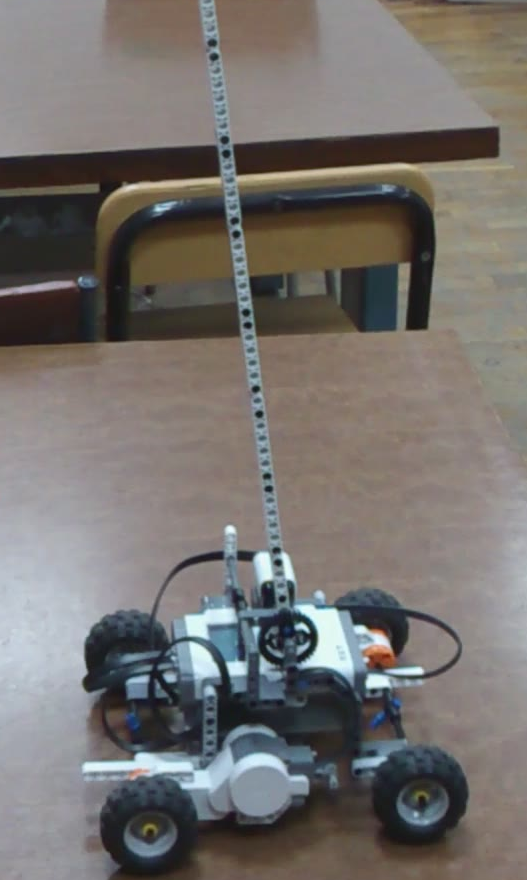
\includegraphics[scale=0.4]{robot.png} }
	\caption{Пример создаваемого робота.}
	\label{robot}
\end{figure}

\paragraph*{Обратный (перевернутый) маятник}$\phantom{-}$\\
\hspace*{\parindent}Любой физический маятник\footnote{Физический маятник~--- маятник, у которого колеблющаяся часть представлена некоторым твердым телом, а сила, вызывающая его движение~--- силой тяжести.}\!\!, имеет два положения равновесия, которые называются \textit{устойчивым} и \textit{неустойчивым} (рис.~\ref{pendulum}).
В~обоих все действующие на маятник силы ($m\vec g$~--- сила тяжести, $\vec N$~--- сила реакции шарнира) уравновешивают друг друга, поэтому, не подвергаясь внешнему воздействию, он пробудет в любом из них бесконечно долго.

\begin{figure}[h]
	\begin{minipage}[h]{0.49\linewidth}
		\center{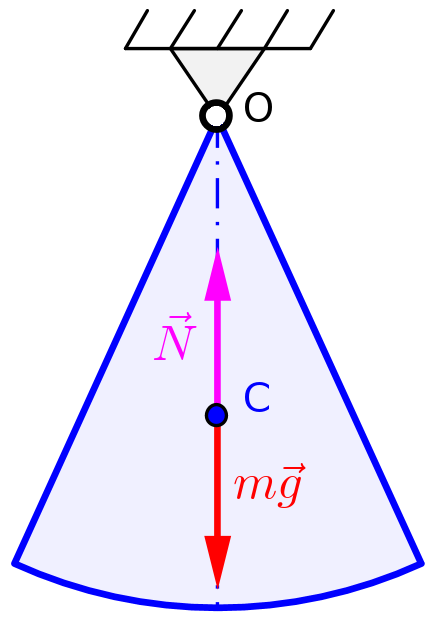
\includegraphics[height = 6 cm]{pendulum.png} \\ а)}
	\end{minipage}
	\hfill
	\begin{minipage}[h]{0.49\linewidth}
		\center{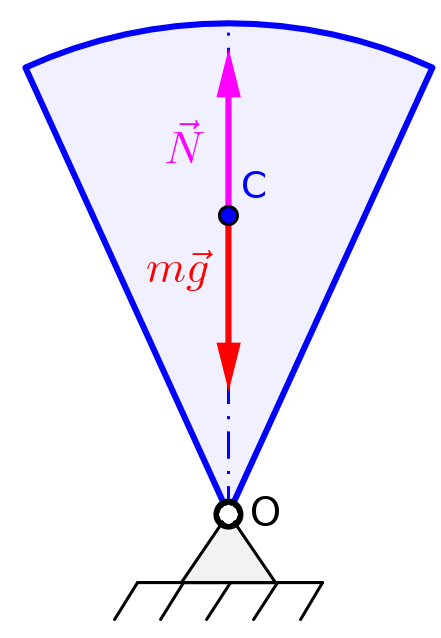
\includegraphics[height = 6 cm]{inverted_pendulum.png} \\ б)}
	\end{minipage}
	\caption{Положения равновесия физического маятника: a)~устойчивое; б)~неустойчивое.}
	\label{pendulum}
\end{figure}

Несмотря на внешнее сходство, достаточно очевидно, что эти положения имеют одно серьезное отличие.
Оно заключается в том, что при выведении маятника из состояния, показанного на рис.~\ref{pendulum}а, он начнет колебаться\footnote{Ко всему прочему благодаря действующим в любой системе силам трения совершаемые им колебания будут затухающими.} относительно своего первоначального положения, то есть не удалится из него, а вот при выведении маятника из состояния, изображенного на рис.~\ref{pendulum}б, он в свою первоначальную позицию уже не вернется.

\begin{figure}[h]
	\begin{minipage}[h]{0.49\linewidth}
		\center{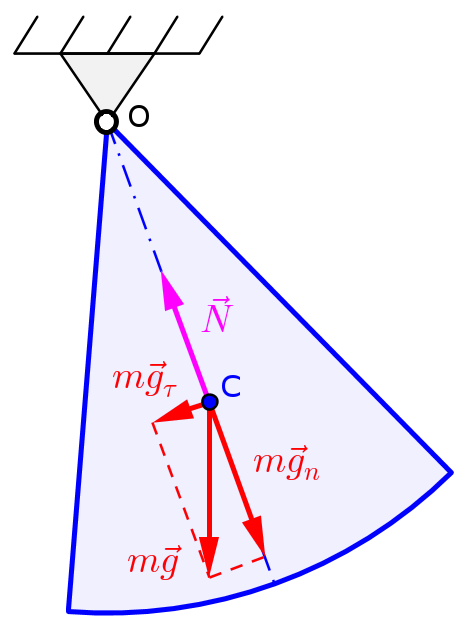
\includegraphics[height = 6 cm]{pendulum_with_angle.png} \\ а)}
	\end{minipage}
	\hfill
	\begin{minipage}[h]{0.49\linewidth}
		\center{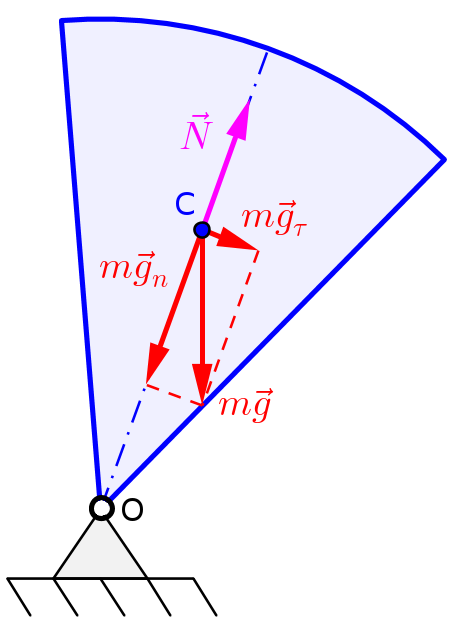
\includegraphics[height = 6 cm]{inverted_pendulum_with_angle.png} \\ б)}
	\end{minipage}
	\caption{Промежуточные положения физического маятника.}
	\label{pendulum_with_angle}
\end{figure}

Такое поведение маятника объясняется направлением силы $m\vec g_\tau$, появляющейся при отклонении маятника из положений равновесия: в первом случае она будет направлена в сторону положения равновесия, а во втором~--- от нее (рис.~\ref{pendulum_with_angle}).
Указанная сила не является самостоятельной, а представляет из себя лишь составляющую силы $m\vec g$, направленную по касательной к траектории движения центра масс тела.

Вопреки сказанному бывает необходимым застабилизировать маятник именно в неустойчивом состоянии.
Это достигается либо непосредственным воздействием на его тело некоторой силой, либо ускоренным перемещением шарнира, к которому он прикреплен.
В~последнем случае (рис.~\ref{inverted_pendulum_with_force}), как известно, относительно своей точки опоры маятник будет вести себя так, как будто испытывает действие силы $m\vec a$ ($\vec a$~--- упомянутое ускорение), направленной в сторону, противоположную перемещению шарнира. При этом тот эффект (или явление), которое получается в результате указанных действий~--- маятник, колеблющийся относительно своего положения неустойчивого равновесия~--- и называется \textit{обратным маятником}.

\begin{figure}[h]
	\noindent\centering{ 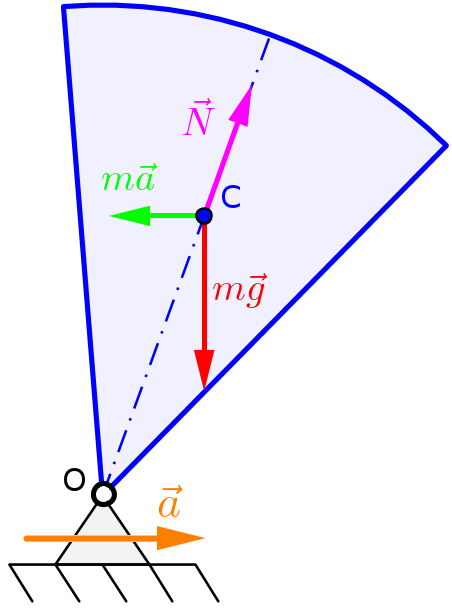
\includegraphics[height = 6 cm]{inverted_pendulum_with_force.png} }
	\caption{Пример удерживающего воздействия.}
	\label{inverted_pendulum_with_force}
\end{figure}

В~этой версии данной лабораторной работы предлагается реализовать модель как раз такого устройства.
При этом задача сводится к тому, чтобы собрать на основе все того же конструктора LEGO Mindstorms маятник-палочку и поместить его на подвижное основание, представляющее из себя четырехколесную полноприводную тележку.
Благодаря специально разработанному алгоритму, последняя, ускоренно перемещаясь, должна уметь удерживать маятник в неустойчивом положении.

\paragraph*{Описание состояния исследуемого устройства}$\phantom{-}$\\
\hspace*{\parindent}Предположим, что <<тело>> нашего робота уже собрано.
В~таком случае согласно материалам прошлых работ следующим шагом должно стать составление его математической модели.

Для этого в первую очередь определим те величины, которые описывают положение робота в пространстве.

Поместим исследуемый механизм в прямоугольную систему координат.
Поскольку его движения будут происходить только вдоль некоторой прямой, то, во-первых, для описания происходящих в нем изменений хватит всего одной координатной плоскости (пусть ею будет $XOY$), а, во-вторых, каждое из входящих в робот тел можно будет рассматривать как лежащую в ней плоскую фигуру, что мы и сделаем. 
В~итоге с учетом всех замечаний получим то, что представлено на рис.~\ref{double_cart_in_decart}.

\begin{figure}[h]
	\noindent\centering{ 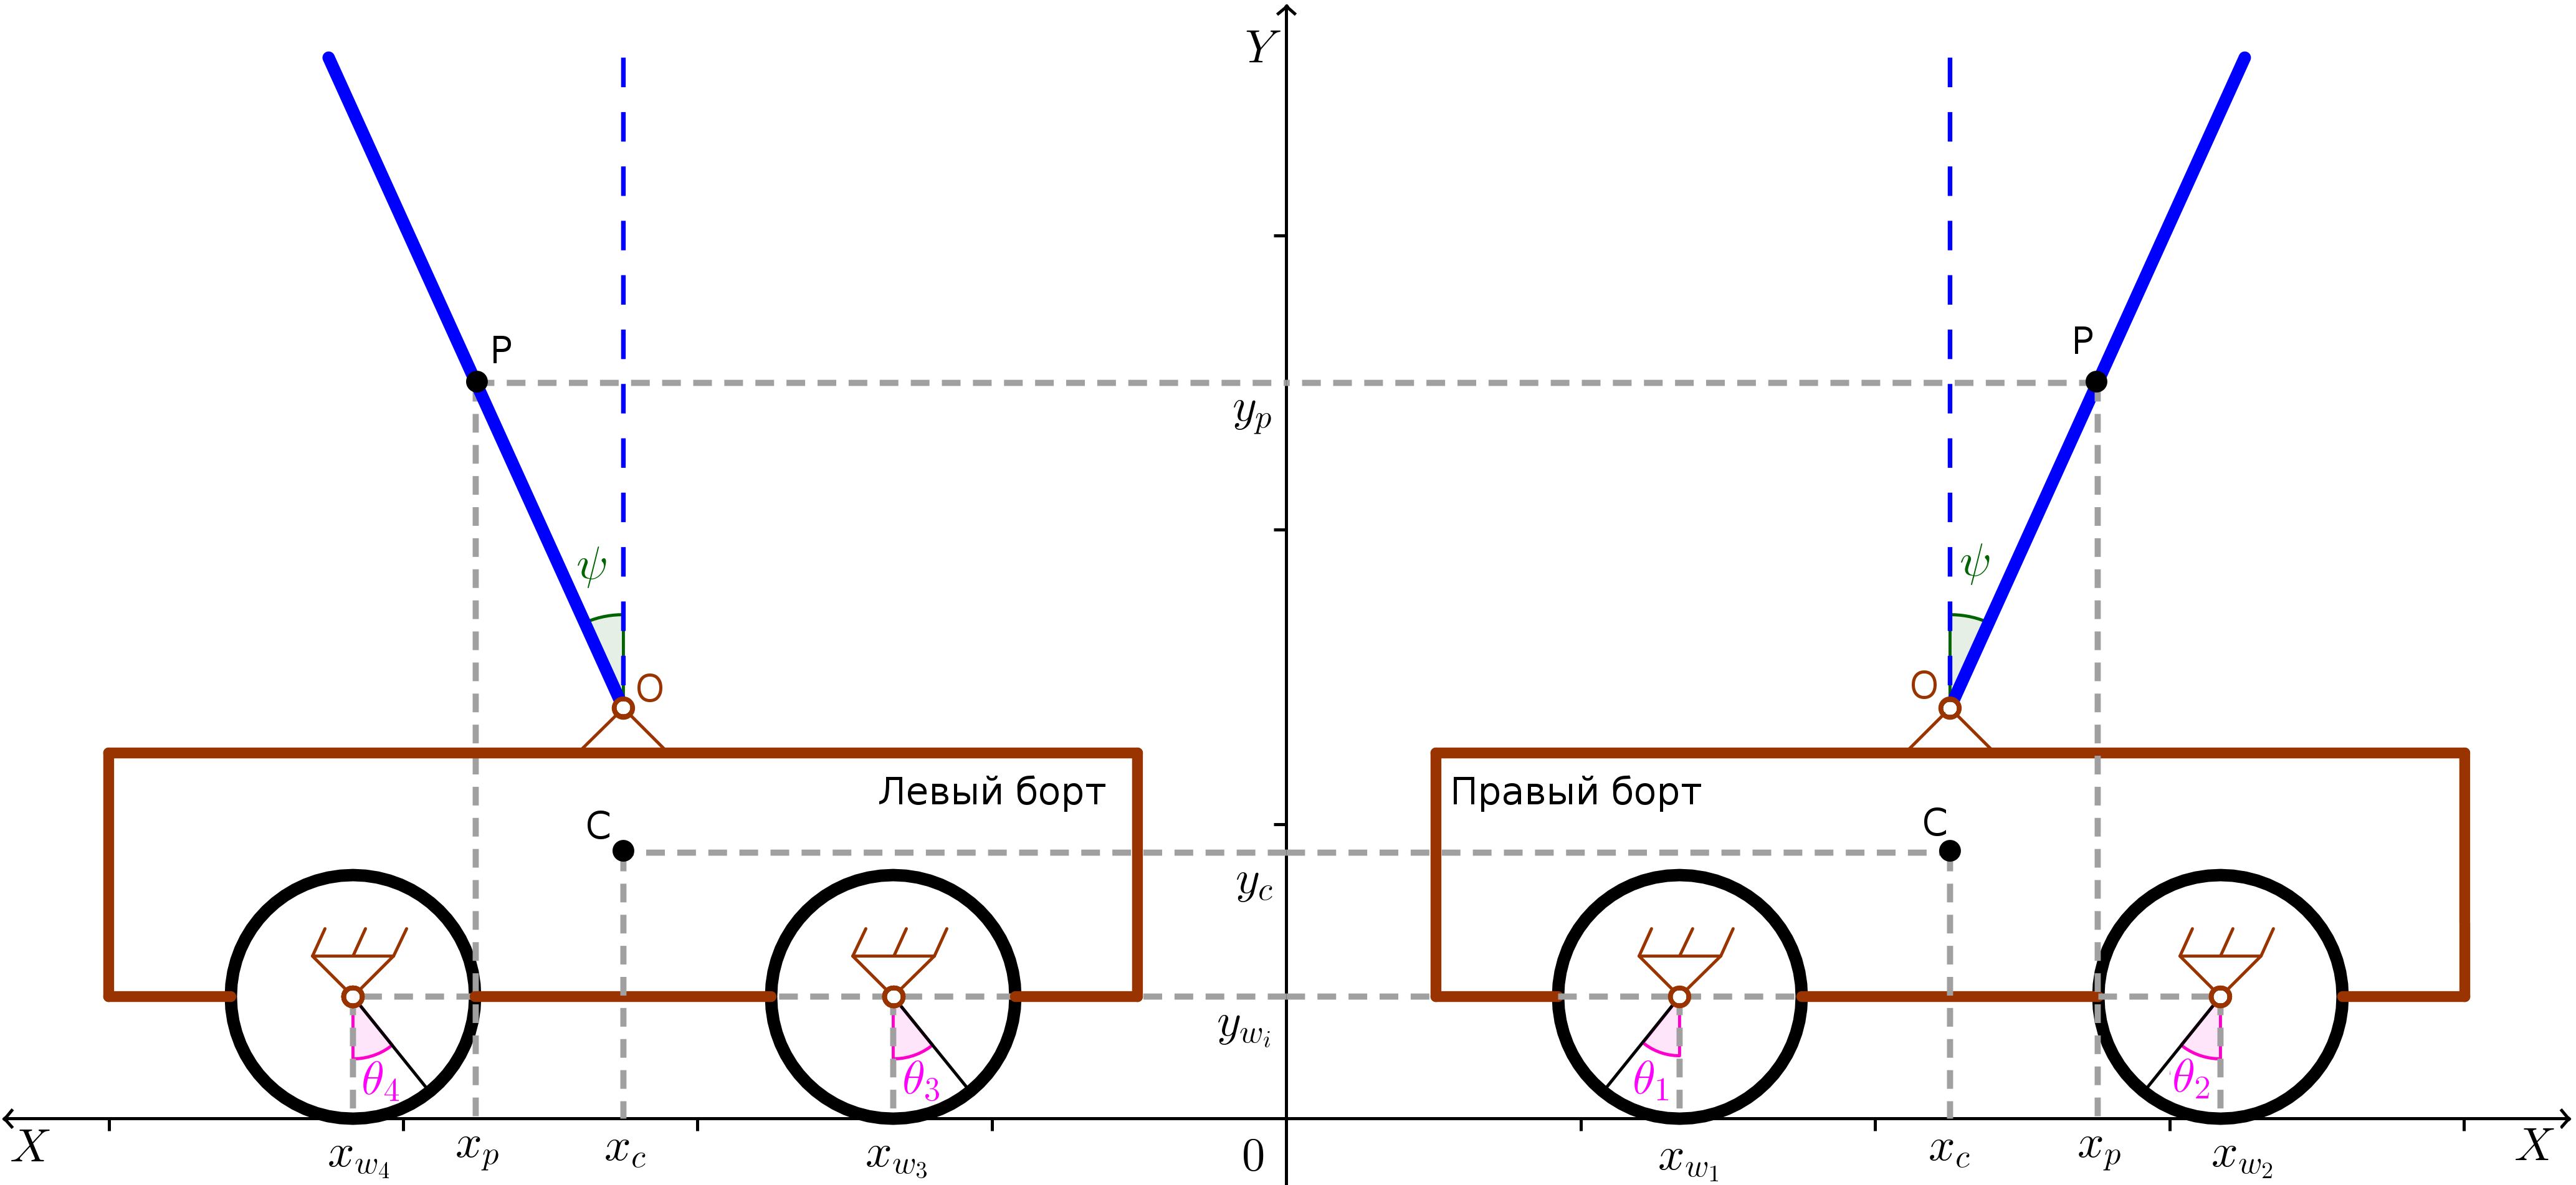
\includegraphics[scale=1]{double_cart_in_decart.png} }
	\caption{Проекции робота в прямоугольную систему координат.}
	\label{double_cart_in_decart}
\end{figure}

Как известно, любая геометрическая фигура, отличная от точки, обладает тремя \textit{степенями свободы}, то есть ее положение в плоскости однозначно определяется заданием \underline{как минимум} каких-либо трех величин\lefteqn.\footnote{\label{snoska}Положение любой плоской фигуры однозначно определяется положениями двух ее точек. 
В~свою очередь, положение каждой точки задается указанием ее декартовых координат~--- двух чисел.
Из сказанного, на первый взгляд, кажется, что положение фигуры в таком случае будет определятся $2+2=4\text{-мя}$ величинами, а значит она будет иметь четыре степени свободы.
Однако, поскольку у недеформируемого тела координаты любых двух его точек, находящихся на расстоянии $d$ друг от друга, связаны известным соотношением
\begin{equation}\label{in_snoska}
	(x_1 - x_2)^2 + (y_1 - y_2)^2 = d^2\!\!,
\end{equation}
позволяющим найти величину одной из координат по значениям остальных, получается, что для фигуры можно определять значение всего трех из четырех характеризующих ее положение величин.
Последнее же и означает, что плоская фигура на плоскости обладает тремя степенями свободы.}
Обычно в их роли выступают декартовы координаты одной из точек рассматриваемой фигуры и некоторый угол, происхождение которого может быть самым разнообразным.

Наш робот состоит из шести тел: четырех колес, маятника и тележки~--- и, как следует из выше сказанного, положение каждого из них должно характеризоваться тремя какими-либо величинами.
Определимся в качестве таковых взять координаты их центров масс $\bigl((x_{w_i},\text{ }y_{w_i})$, $(x_c,\text{ }y_c)$ и $(x_p,\text{ }y_p)$, где $i\in\{1,2,3,4\}\bigr)$ и углы: на который он отклоняется от вертикали~--- для маятника ($\psi$); на который она поворачивается из первоначального положения~--- для тележки ($\zeta$; не обозначен на рис.~\ref{double_cart_in_decart} по причинам, которые будут указаны ниже); на который они поворачиваются из первоначального положения~--- для колес ($\theta_i$).
Несложно видеть, что в таком случае сам робот (все входящие в него тела вместе взятые) описывается $3 \cdot 6 = 18\text{-ью}$ величинами.

Заметим, что иногда определенное таким способом количество координат, характеризующих исследуемый механизм, оказывается избыточным.
Это происходит в том случае, если взаимодействие составляющих его тел друг с другом или с другими телами приводит к тому, что на движения или положения первых налагаются определенные ограничения.
Они, называемые \textit{связями}\lefteqn,\footnote{Иногда под \textit{связями} подразумевают не сами ограничения, а создающие их тела, например нити, балки и~т.д.} в общем случае выражаются в том, что значения координат или скоростей рассматриваемых тел не могут быть любыми, а должны подчиняться определенным количественным соотношениям.
При всем этом интересующие нас ситуации, в которых количество степеней свободы рассматриваемого механизма оказывается меньшим, чем сумма количеств степеней свободы, входящих в него тел, возникают тогда, когда эти соотношения касаются только координат и могут быть записаны в виде некоторых равенств, подобных выражению~\eqref{in_snoska}\footnote{Помимо указанных существуют и иные связи, приводящие к уменьшению количества степеней свободы, однако в данном курсе о них говорится не будет.}\!\!.

А теперь поясним сказанное на примере нашего робота, для которого количество степеней свободы (говорим, забегая вперед) оказывается на самом деле меньшим 18-ти.

Первая связь, наблюдаемая в нашей модели, создается шарниром, соединяющим маятник и тележку.
Ее существование сказывается на том, что положение этих тел относительно друг друга не может быть произвольным.
Математически она записывается в виде двух уравнений:
\begin{gather}
	x_p = x_c + |OP|\sin\psi\\
	y_p = y_c + |OC| + |OP|\cos\psi
\end{gather}   
где $|OP|$ и $|OC|$~--- длины отрезков $OP$ и $OC$ соответственно (последний подразумевается параллельным оси $OY$).
Если учесть, что центр масс тонкого однородного стержня находится в его середине, то есть
\begin{equation}
	|OP| = \frac{l}{2},
\end{equation} 
где $l$~--- длина маятника, то данные выражения можно переписать в виде
\begin{gather}
	x_p = x_c + \frac{l}{2}\sin\psi \label{xp}\\
	y_p = y_c + |OC| + \frac{l}{2}\cos\psi\ldotp \label{yp} 
\end{gather}   
Полученные соотношения позволяют по известным значениям трех из пяти встречающихся в них величин в любой момент времени вычислять остальные две.
Следовательно, для того чтобы описать состояние механизма в любой момент времени, две координаты можно не узнавать непосредственно, а рассчитывать по полученным выражениям исходя из значений остальных.
Это, в свою очередь, говорит о том, что две величины становятся лишними, а значит указанная связь снижает предполагаемое количество степеней свободы механизма на две~--- до 16-ти.  
Условимся <<отбросить>> $x_p$ и $y_p$.

Следующая порция связей оказывает непосредственное влияние на колеса робота.
В~нее входят, во-первых, связи создаваемые плоскостью, по которой движется механизм, во-вторых, связи, создаваемые осями, которые объединяют колеса в пары, и, в-третьих, те, которые создаются крепежными элементами, соединяющими колеса с тележкой.
В~конечном итоге их существование вызывает следующие очевидные последствия:
\begin{itemize}
	\item Все колеса, катясь, перемещаются по одной и той же горизонтальной плоскости. 
	Это приводит к тому, что ординаты центров масс всех колес будут одинаковыми и равными, например, $y_w$\lefteqn.\footnote{Это свойство стало причиной того, что на рис.~\ref{double_cart_in_decart} было дано лишь их общее обозначение~--- $y_{w_i}$.}
	Однако несложно видеть, что при движении тележки координата $y_w$ меняться не будет ($y_w = const$), а следовательно, нет необходимости каждый раз находить и ее. 
	Действительно, ведь, измерив ее единожды, в дальнейшем значение $y_w$ будет известным в любой момент времени.
	
	Таким образом, имеем, что из рассмотрения выбывают еще четыре степени свободы, которые ранее были представлены координатами $y_{w_i}$, где $i\in\{1,2,3,4\}$.
	\item Все колеса, катясь, движутся в плоскостях, параллельных введеной нами плоскости $XOY$, следовательно центры масс тех из них, которые являются соосными, будут обладать одинаковыми абсциссами. 
	Математически это можно записать как 
	\begin{gather}
		x_{w_1} = x_{w_3} = x_{w_1}^*, \\
		x_{w_2} = x_{w_4} = x_{w_2}^*,
	\end{gather}
	где $x_{w_1}^*$ и $x_{w_2}^*$~--- просто новые обозначения.
	Данные выражения показывают, что указанная особенность вычитает еще две степени свободы, и их общее количество сокращается до 10-ти.
	\item Соосные колеса в любой момент времени будут характеризоваться одинаковыми  значениями углов поворота из начального положени, следовательно аналогичные прошлым выражения:
	\begin{gather}
		\theta_1 = \theta_3 = \theta_1^*, \\
		\theta_2 = \theta_4 = \theta_2^*
	\end{gather}
	~--- покажут, что рассмотренная связь уменьшит <<оставшееся>> количество степеней свободы еще на два.
\end{itemize}

Тележка, входящая в состав робота, также испытывает влияние связей.
Одна из них, которая, впрочем, уже рассматривалась, будет действовать со стороны шарнира, соединяющего тележку с маятником, остальные~--- со стороны крепежных элементов, соединяющих ее с колесами.
В~итоге совокупное действие этих связей приводит к тому, что тележка при своем движении, во-первых, не поворачиватся относительно первоначального состояния\lefteqn,\footnote{Это, к слову сказать, является причиной того, что на приводимых рисунках не отмечался угол $\zeta$} а во-вторых, не перемещается по вертикали.
Сказанное, как уже можно догадаться, означает, что ответственные за отмеченные особенности величины (угол $\zeta$ и ординату $y_c$) также можно вывести из рассмотрения. 

Опираясь на последствия существования выше описанных связей, к данному моменту мы установили, что количество степеней свободы нашего робота, скорее всего, будет равно шести.
До сих пор оставшиеся актуальными величины, характеризующие его состояние, показаны на рис.~\ref{cart_in_decart}.
Однако необходимо заметить, что настоящее количество степеней свободы окажется еще меньшим.

\begin{figure}[h]
	\noindent\centering{ 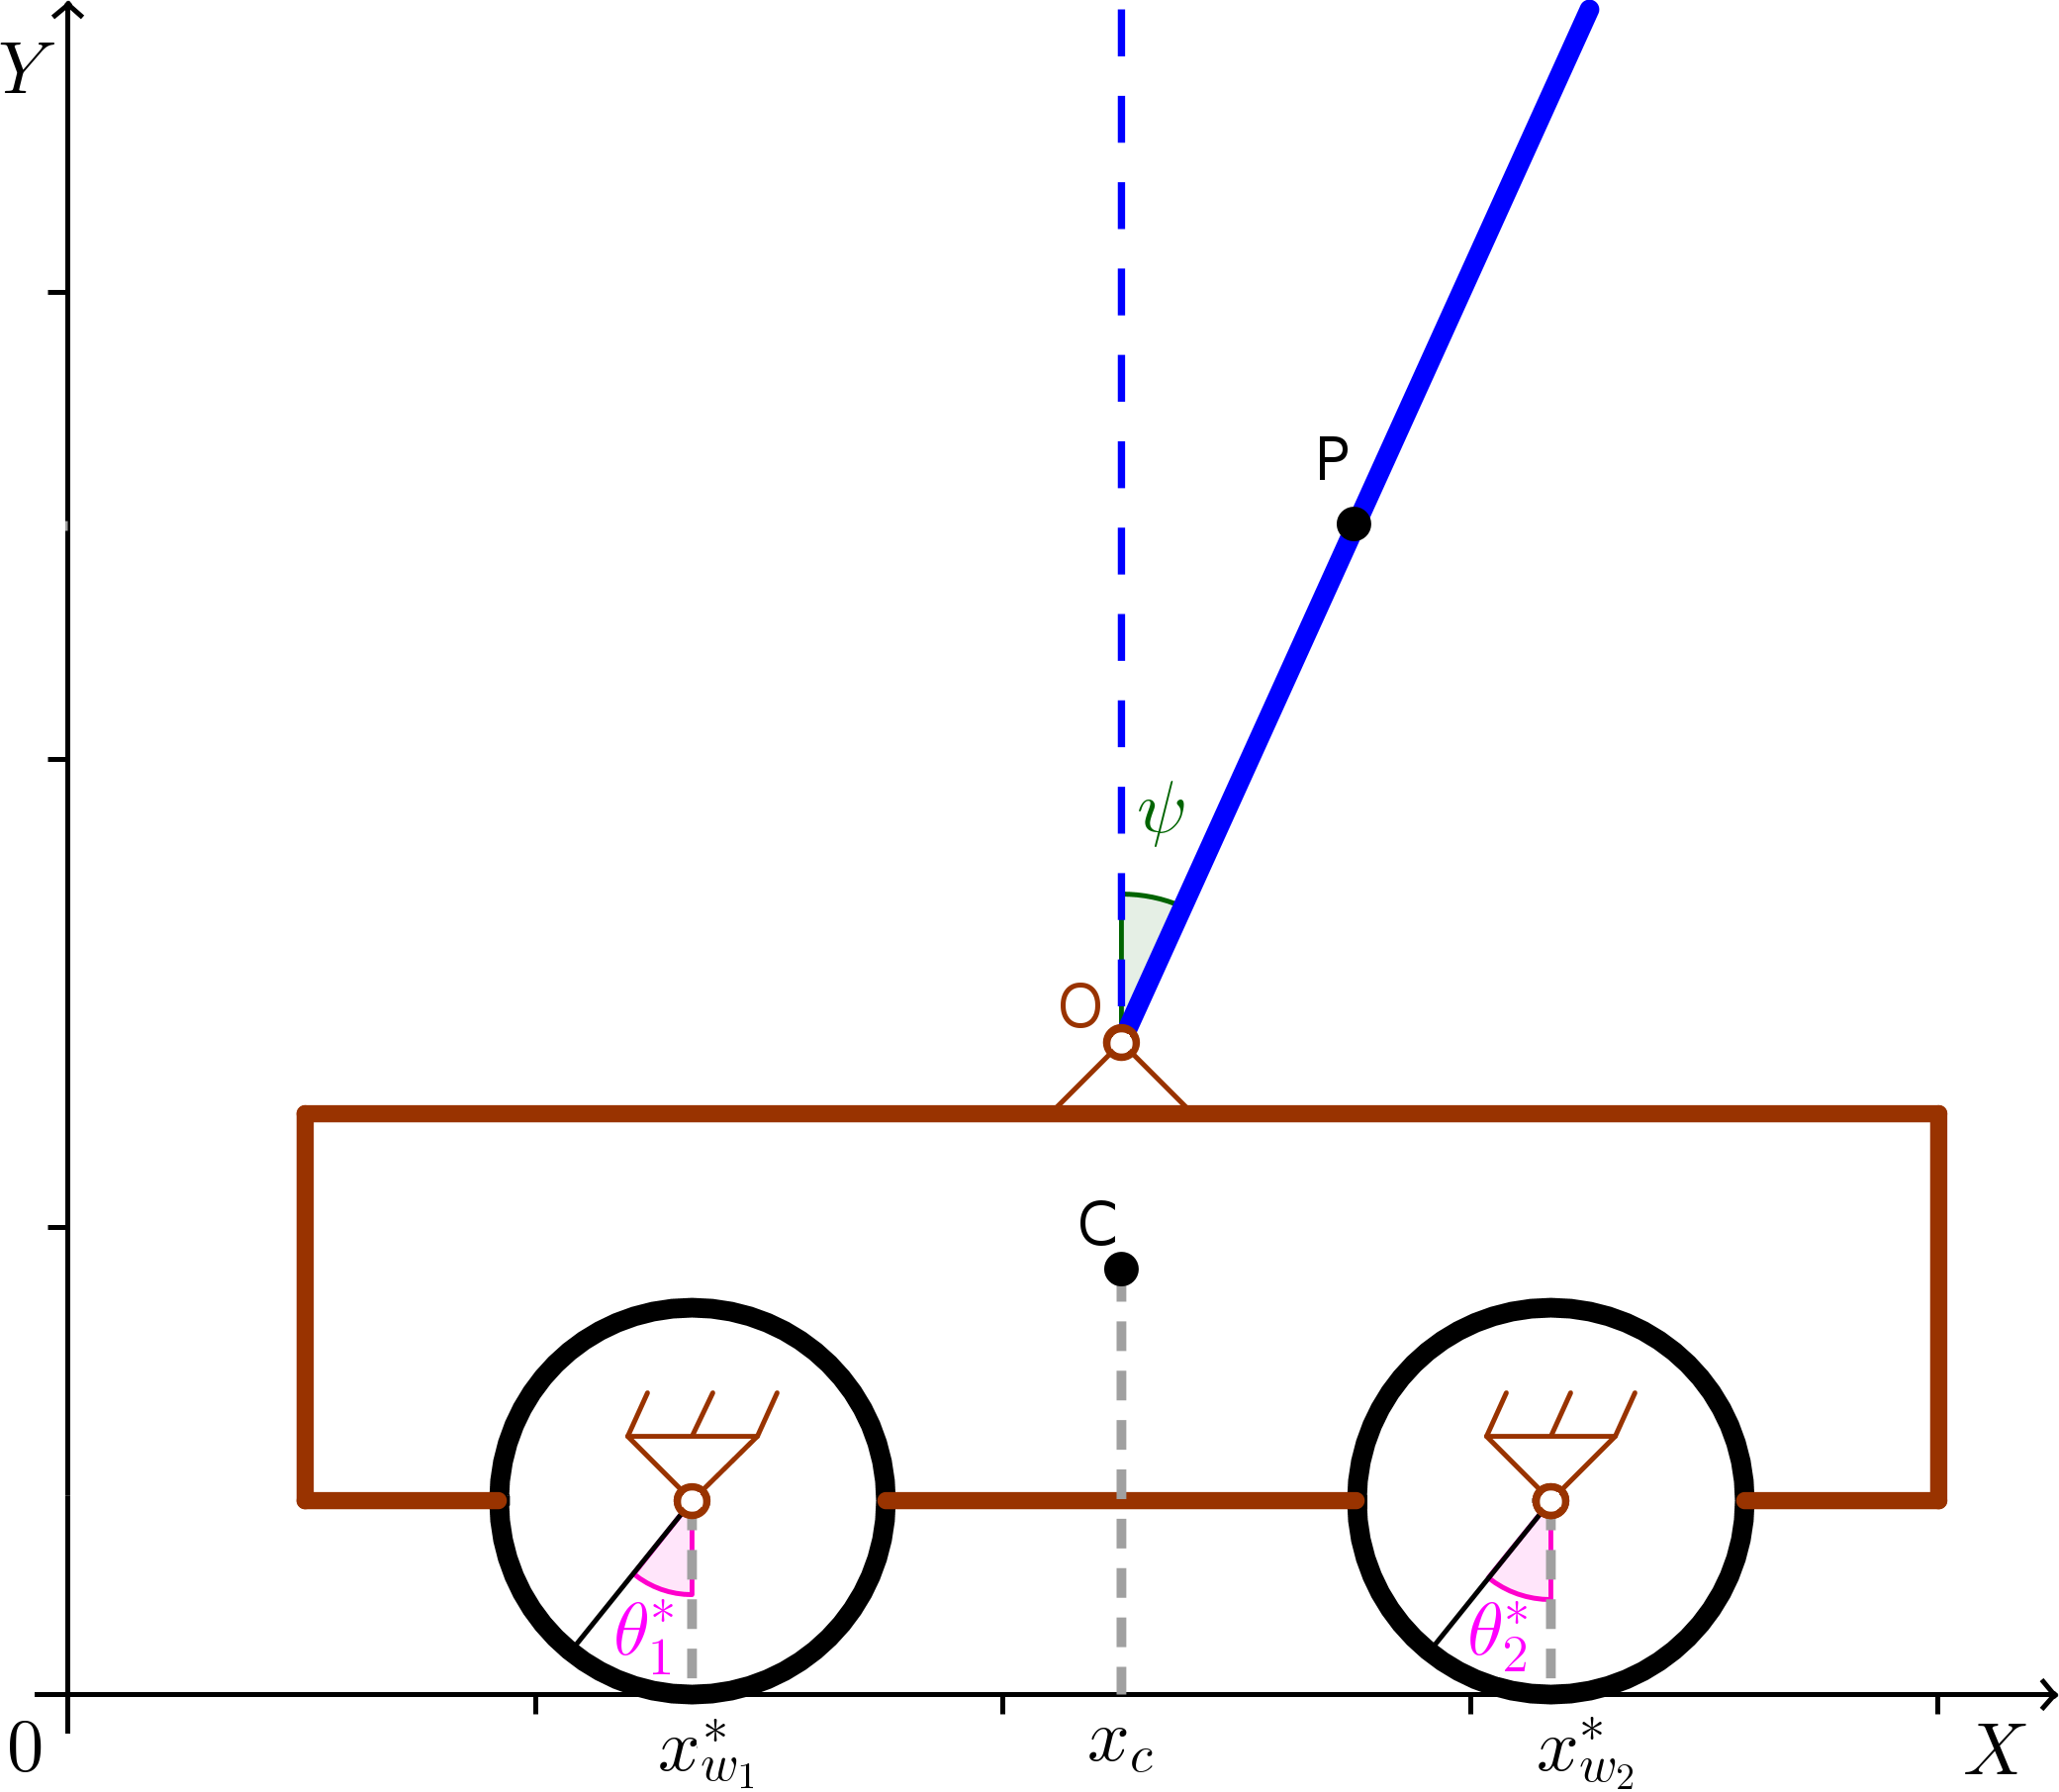
\includegraphics[scale=1]{cart_in_decart.png} }
	\caption{Неисключенные величины и их физический смысл.}
	\label{cart_in_decart}
\end{figure}

Дело в том, что ряд оставшихся величин позволят исключить те связи, которые являются следствием недеформируемости входящих в робот тел и постоянства расстояний между их различными точками\lefteqn.\footnote{Похожая ситуация рассматривалась в сноске~\ref{snoska}.}
Например, из-за указанных особенностей абсциссы центров масс колес и тележки будут удовлетворять выражениям
\begin{gather}
	x_{w_2}^* - x_c = const\label{in_constant1}\\
	x_c - x_{w_1}^* = const\label{in_constant2},
\end{gather}
которые позволят вывести из рассмотрения еще две координаты (пусть ими будут $x_{w_1}^*$ и $x_{w_2}^*$) и сократить прогнозируемое количество степеней свободы механизма до 4-ех.

Достигнув этого момента, надо сказать, что никакие дальнейшие поиски связей не приведут ни к какому результату, а следовательно количество степеней свободы нашего робота на самом деле равно 4-ем.
Однако, если рассмотреть частный случай, предположив, что при движении механизма его колеса не проскальзывают относительно поверхности\lefteqn,\footnote{С точки зрения кинематики это означает, что при движении колеса точки, по которым оно и поверхность касаются друг друга, будут иметь равные скорости.} по которой он движется, можно получить еще две связи.
Первая из них заключается в том, что углы поворота всех колес будут равны между собой:
\begin{equation}
	\theta_1^* = \theta_2^* = \theta, 
\end{equation}
где $\theta$~--- просто новое обозначение, а вторая приводит к тому, что перемещение робота ($d$) будет связано с углом $\theta$ выражением\footnote{Поскольку <<дорожное покрытие>> покоится, скорость любой ее точки равна нулю. 
С~учетом того, что точки, по которым колесо и <<дорога>> касаются друг друга (на рис.~\ref{wheel} это точка $A'$), движутся с одинаковой скоростью, получаем, что скорость точки $A'$ также будет равна нулю ($v_a=0$).

С~другой стороны, скорость точки $A'$, согласно преобразованиям Галилея, равна сумме скорости центра масс ($\vec v$) колеса и скорости движения точки $A'$ относительно последнего ($\vec v_{ac}$), т.е. $\vec v_a=\vec v+\vec v_{ac}$. Поскольку относительно центра масс точка $A'$ совершает чисто вращательное движение c угловой скоростью $\omega$, то $v_{ac}=\omega\cdot r$ и $\vec v_{ac}\uparrow\downarrow\vec v$. Собрав все наблюдения воедино, получим, что $v = \omega r$. Из последнего же равенства и следует выражение~\eqref{d=rtheta}.} 
\begin{equation}\label{d=rtheta}
	d = r\theta,
\end{equation}
где $r$~--- радиус колеса (рис.~\ref{wheel}). 
Последнее уравнение с учетом выражения 
\begin{equation}
	x_c = d + x_c^{(0)}\!,
\end{equation}
где $x_c^{(0)}$~--- значение $x_c$ в начальный момент времени, позволяет заключить, что
\begin{equation}\label{xc}
	x_c = x_c^{(0)} + r\theta\ldotp
\end{equation}

\begin{figure}[h]
	\noindent\centering{ 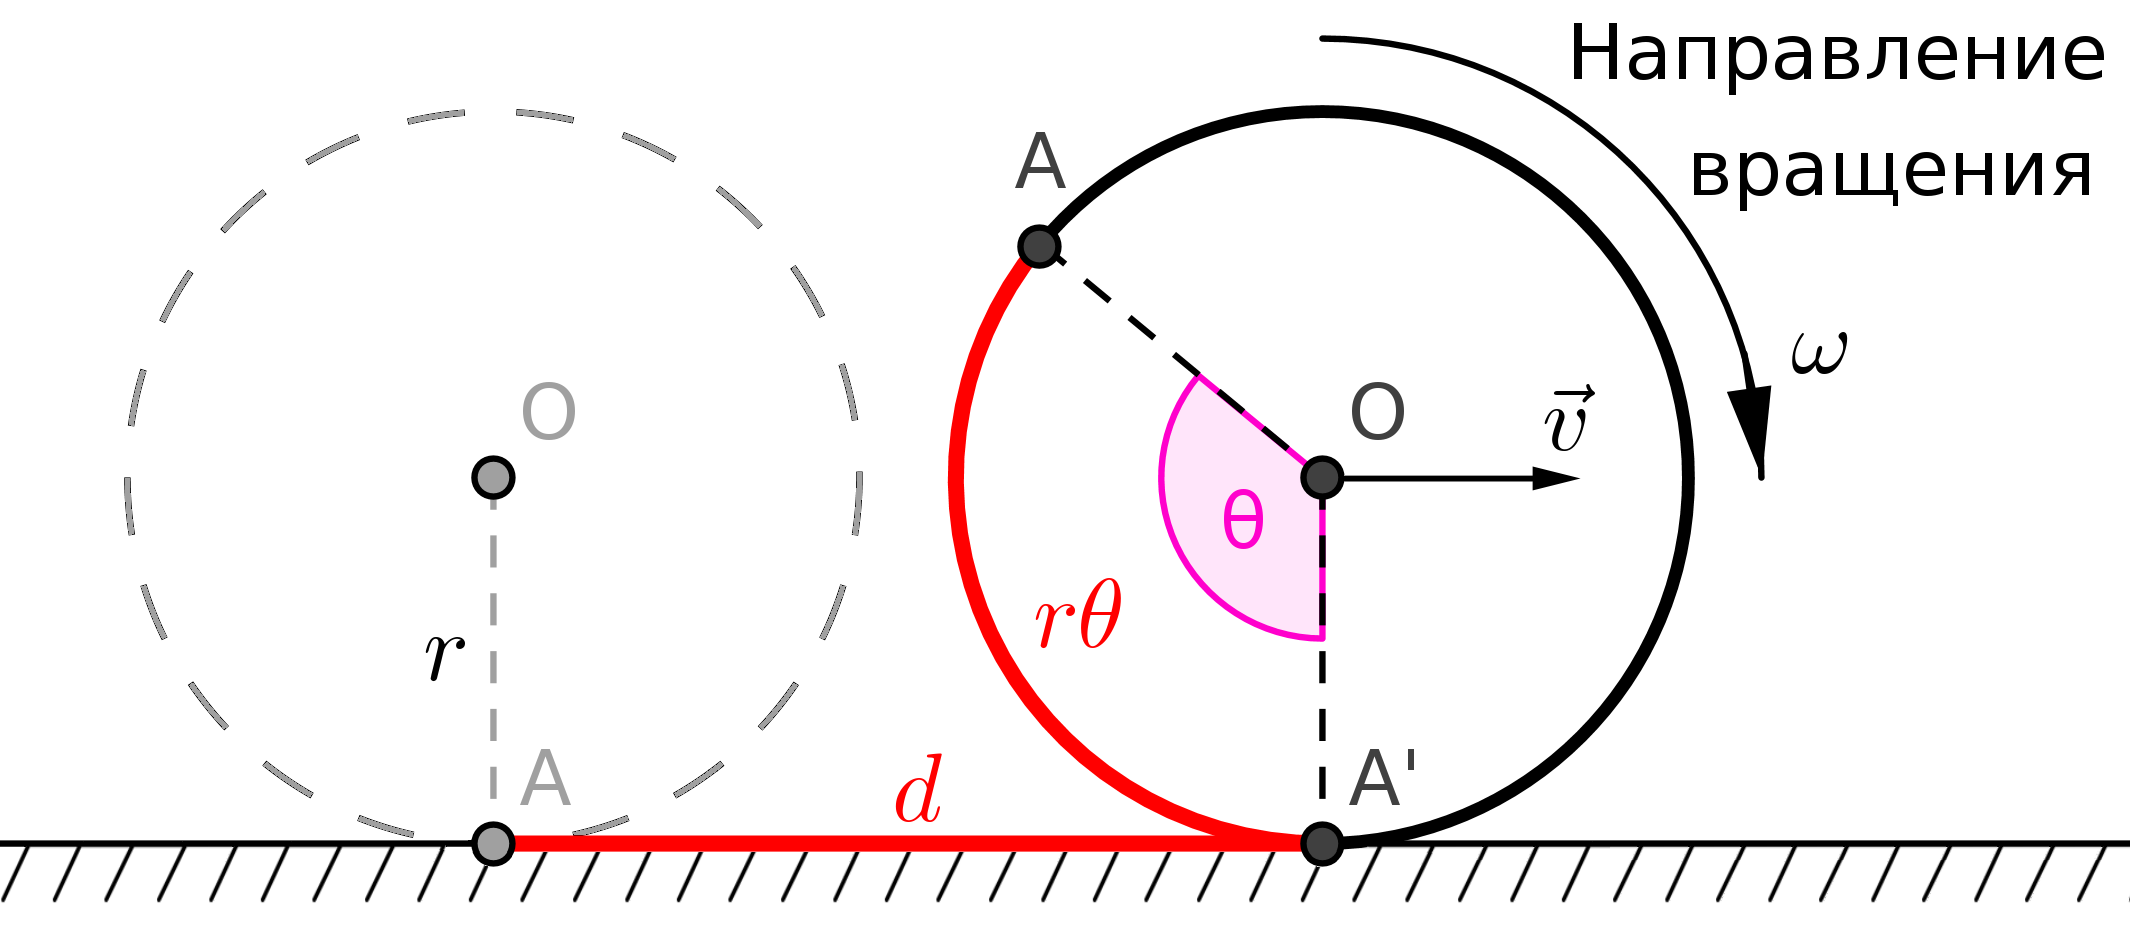
\includegraphics[scale=1.2]{wheel.png} }
	\caption{Движение колеса без проскальзывания.}
	\label{wheel}
\end{figure}

Очевидно, что в таком случае первая связь позволит отбросить величины $\theta_1^*$ и $\theta_1^*$, заменив их одним углом $\theta$, а вторая~--- абсциссу $x_c$.
Таким образом, имеем, что исследуемый механизм имеет всего две степени свободы, выражающиеся в нашем случае углами $\theta$ и $\psi$\lefteqn.\footnote{Еще раз подчеркнем, что можно было бы выбрать и другую пару координат.}

В~заключение важно отметить, что подобные углам $\theta$ и $\psi$ величины носят название \textit{обобщенных координат}.
Именно о них упоминалось в тексте лабораторной работы~№1.

\paragraph*{Уравнения движения робота}$\phantom{-}$\\
\hspace*{\parindent}Теперь, после того, как для робота были определены характеризующие его состояние величины, настало время написания соответствующих уравнений.
Всего предстоит раскрыть две стороны его работы~--- механическую и электродинамическую.

Начнем с первой.
Подобно тому, как это было сделано в работе~№1, сначала мы воспользуемся законами Ньютона, а уже потом~--- уравнениями Лагранжа.

\begin{figure}[h]
	\noindent\centering{ 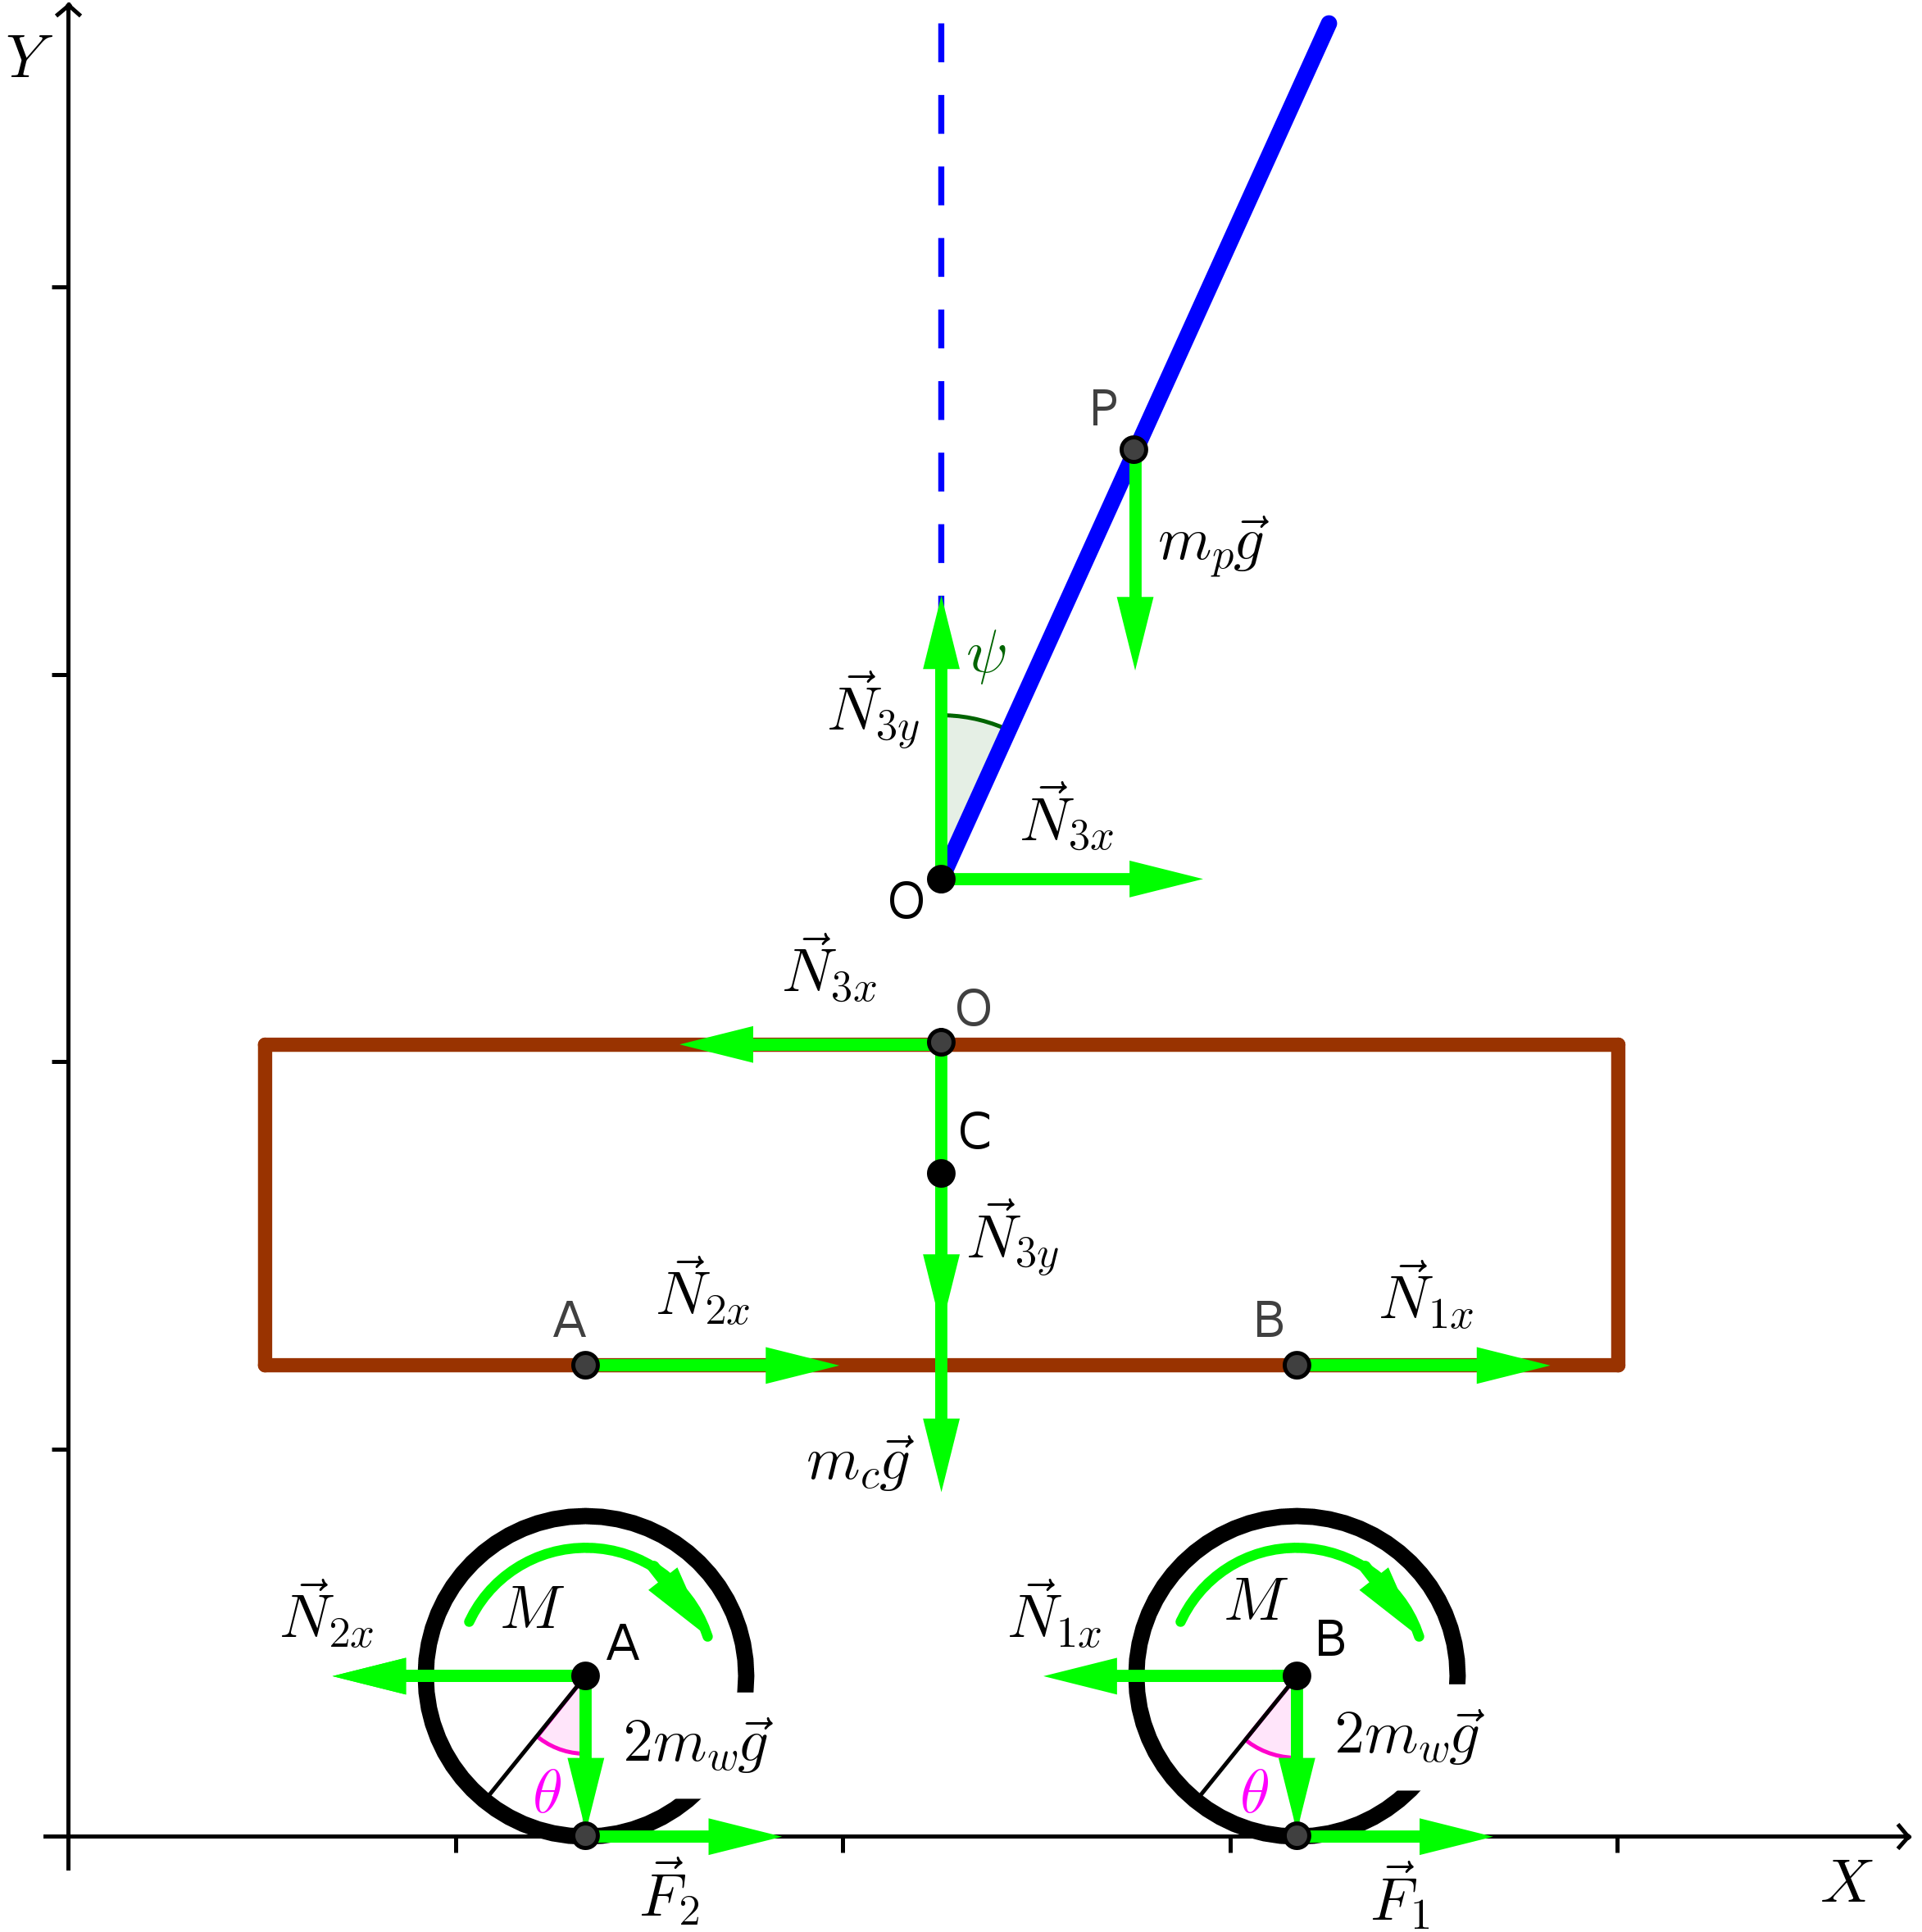
\includegraphics[scale=1.2]{forces.png} }
	\caption{Действующие в системе силы.}
	\label{forces}
\end{figure}

Согласно одному из подходов к описанию движения твердых тел, для того чтобы полностью охарактеризовать поведение исследуемого тела, надо составить уравнения второго закона Ньютона для его вращательного и поступательного движений.
При этом для написания уравнений, описывающих его поступательное движение, тело следует принять за материальную точку, а при определении уравнений вращательного движения моменты всех сил и момент инерции самого тела следует отсчитывать от его центра масс. 
В таком случае, отметив силы, действующие в нашем механизме (рис.~\ref{forces}; отмечены не все силы, действующие в системе, а только те, которые потребуются), получим\footnote{Все входящие в приведенные ниже уравнения величины, которые могут каким-либо образом зависеть от времени, считайте таковыми.}\\
для маятника:
\begin{align}
	&m_p\ddot{x}_p = N_{3x},\label{mpax} &&\text{(2-ой закон в проекциях на ось $OX$)}\\
	&m_p\ddot{y}_p = N_{3y} - m_pg,\label{mpay} &&\text{(2-ой закон в проекциях на ось $OY$)}\\
	&J_p\ddot{\psi} = N_{3y}\frac{l}{2}\sin\psi - N_{3x}\frac{l}{2}\cos\psi; \label{Jpe} &&\text{(уравнение моментов)}	
	\intertext{для тележки:}
	&m_c\ddot{x}_c = N_{1x} + N_{2x} - N_{3x}; \label{mcax} &&\text{(2-й закон в проекциях на ось $OX$)}\\
	\intertext{для одной пары колес:}
	&2m_w\ddot{x}_{w_1}^* = F_1 - N_{1x}, \label{mw1ax} &&\text{(2-й закон в проекциях на ось $OX$)}\\
	&2J_w\ddot{\theta} = M - F_1r \label{Jw1}; &&\text{(уравнение моментов)}
	\intertext{для другой:}
	&2m_w\ddot{x}_{w_2}^* = F_2 - N_{2x}, \label{mw2ax} &&\text{(2-й закон в проекциях на ось $OX$)}\\
	&2J_w\ddot{\theta} = M - F_2r \label{Jw2}, &&\text{(уравнение моментов)}
\end{align}
где $N_1$ и $N_2$~--- силы реакции, возникающие между тележкой и разными парами соосных колес (индексами помечены их проекции на соответствующие оси); $N_3$~--- сила реакции, возникающая между маятником и тележкой;  $F_1$ и $F_2$~--- силы трения возникающие между парами соосных колес и <<дорожным покрытием>> (аналогичные силы приводят в движение автомобили); $M$~--- вращательный момент, с которым мотор NXT действует на колеса; $m_w$~--- масса одного колеса; $m_p$~--- масса маятника; $m_c$~--- масса тележки;  $J_p$~--- момент инерции маятника; $J_w$~--- момент инерции колеса; $g$~--- ускорение свободного падения.

Комментируя полученные уравнения можно сказать слеующее.
Во-первых, как мы уже отмечали ранее, соосные колеса обладают одинаковыми кинематическими характеристиками.
По этой причине уравнения движения составлены сразу для их пар, а не для отдельных колес.
Это объясняет, почему перед величинами $m_w$ и $J_w$ стоят множители, равные двум.
Во-вторых, важно отметить то, что при написании уравнений подразумевалось, что в конструкцию робота входят два двигателя NXT: первый подает силовое воздействие на одну пару колес, второй~--- на другую, как на рис.~\ref{robot}.
Это объясняет, почему момент $М$ без всяких числовых коэффициентов присутствует в соответствующих уравнениях для обеих пар колес. 

Для дальнейшего использования полученных уравнений несколько преобразуем их:
\begin{enumerate}
	\item Подставим значение $N_{3x}$ из~\eqref{mpax} и значение $N_{3y}$ из~\eqref{mpay} в уравнение~\eqref{Jpe}:
		\begin{equation}\label{other_from_withoutNs&Fs}
			\left(m_p\ddot{y}_p + m_pg\right)\frac{l}{2}\sin\psi - m_p\ddot{x}_p\frac{l}{2}\cos\psi = J_p\ddot{\psi}\ldotp
		\end{equation}
	\item Сложим уравнения друг с другом уравнения~\eqref{mw1ax} и \eqref{mw2ax}, а также~\eqref{Jw1} и \eqref{Jw2}:
		\begin{gather}
			\!(F_1 + F_2) - (N_{1x} + N_{2x}) = 2m_w(\ddot{x}_{w_1}^* + \ddot{x}_{w_2}^*)\label{Fs&Ns}\\
			\!2M - (F_1 + F_2)r = 4J_w\ddot{\theta}\label{2Ms&Fs}\ldotp
		\end{gather}
	\item Подставим выражение для суммы $(F_1 + F_2)$ из~\eqref{2Ms&Fs} в \eqref{Fs&Ns}:
		\begin{equation}
			N_{1x} + N_{2x} = \frac{2M}{r} - \frac{4J_w}{r}\ddot{\theta} - 2m_w(\ddot{x}_{w_1}^* + \ddot{x}_{w_2}^*)\ldotp\label{Ns}
		\end{equation}
	\item Подставим выражение для суммы $(N_{1x} + N_{2x})$ из~\eqref{Ns} и выражение для $N_{3x}$ из~\eqref{mpax} в уравнение~\eqref{mcax}:
		\begin{equation}\label{withoutNs&Fs}
			\frac{2M}{r} - \frac{4J_w}{r}\ddot{\theta} - 2m_w(\ddot{x}_{w_1}^* + \ddot{x}_{w_2}^*) - m_p\ddot{x}_p = m_c\ddot{x}_c\ldotp	
		\end{equation}
	\item Объединим уравнения~\eqref{withoutNs&Fs} и \eqref{other_from_withoutNs&Fs} в систему:
		\begin{equation}\label{XWs&XCs}
			\left\{
				\begin{aligned}
					\!&\left(m_p\ddot{y}_p + m_pg\right)\frac{l}{2}\sin\psi - m_p\ddot{x}_p\frac{l}{2}\cos\psi = J_p\ddot{\psi}\\
					\!&\frac{2M}{r} - \frac{4J_w}{r}\ddot{\theta} - 2m_w(\ddot{x}_{w_1}^* + \ddot{x}_{w_2}^*) - m_p\ddot{x}_p =
					 m_c\ddot{x}_c\ldotp
				\end{aligned}
			\right.
		\end{equation}
\end{enumerate}

Таким образом, применением законов Ньютона к нашему механизму была получена система уравнений~\eqref{XWs&XCs}.
Несложно видеть, что в то время, как исследуемый робот имеет всего две степени свободы, она содержит сразу семь величин, описывающих положение различных тел в пространстве.
Поскольку такое их количество избыточно, выразим лишние из них через функции $\theta(t)$ и $\psi(t)$, опираясь на ранее полученные уравнения связей:
\begin{enumerate}
	\item Так как, согласно выражениям~\eqref{in_constant1} и \eqref{in_constant2}, функции $x_c(t)$, $x_{w_1}^*(t)$ и $x_{w_2}^*(t)$
		отличаются друг от друга на постоянные величины, можно сделать вывод, что их производные будут равны.
		По этой причине заменим в выражении~\eqref{XWs&XCs} функции $\ddot{x}_{w_1}^*$ и $\ddot{x}_{w_2}^*$ на функцию $\ddot{x}_c$:
		\begin{equation}\label{XCs}
			\left\{
				\begin{aligned}
					\!&\left(m_p\ddot{y}_p + m_pg\right)\frac{l}{2}\sin\psi - m_p\ddot{x}_p\frac{l}{2}\cos\psi = J_p\ddot{\psi}\\
					\!&\frac{2M}{r} - \frac{4J_w}{r}\ddot{\theta} - 4m_w\ddot{x}_c - m_p\ddot{x}_p =
					 m_c\ddot{x}_c\ldotp
				\end{aligned}
			\right.
		\end{equation}
	\item Получим, согласно уравнению~\eqref{xc}:
		\begin{equation}
			\ddot x_c = r\ddot\theta\ldotp
		\end{equation}
	\item Получим из уравнений~\eqref{xc}, \eqref{xp} и \eqref{yp}:
		\begin{gather}
			\ddot x_p = r\ddot\theta - 0.5l\dot\psi^2\sin\psi + 0.5l\ddot\psi\cos\psi,\\
			\ddot y_p = - 0.5l\dot\psi^2\cos\psi - 0.5l\ddot\psi\sin\psi\ldotp
		\end{gather}
	\item Подставим выражения, полученные в двух прошлых пунктах, в систему~\eqref{XCs}:
		\begin{equation}
			\left\{
				\begin{aligned}					
					\!&\begin{split}					
						&\left(m_p\left(- 0.5l\dot\psi^2\cos\psi - 0.5l\ddot\psi\sin\psi\right) + m_pg\right)\frac{l}{2}\sin\psi - \\
						&\phantom{-------}-m_p\left(r\ddot\theta - 0.5l\dot\psi^2\sin\psi + 0.5l\ddot\psi\cos\psi\right)
						\frac{l}{2}\cos\psi = J_p\ddot{\psi}
					\end{split}\\		
					\!&\frac{2M}{r} - \frac{4J_w}{r}\ddot{\theta} - 4m_wr\ddot{\theta} - m_p\left(r\ddot\theta - 0.5l\dot\psi^2\sin\psi 
					+ 0.5l\ddot\psi\cos\psi\right) = m_cr\ddot{\theta},
				\end{aligned}
			\right.
		\end{equation}	
		и упростим полученный результат:
		\begin{equation}\label{from_Newton's_final}
			\left\{
				\begin{aligned}
					\!&-0.25m_pl^2\ddot{\psi} + 0.5m_plg\sin\psi -0.5m_prl\ddot{\theta}\cos\psi= J_p\ddot{\psi}\\				
					\!&\frac{2M}{r} - \frac{4J_w}{r}\ddot{\theta} - 4m_wr\ddot{\theta} - m_pr\ddot\theta + 0.5m_pl\dot\psi^2\sin\psi 
					- 0.5m_pl\ddot\psi\cos\psi = m_cr\ddot{\theta}\ldotp
				\end{aligned}
			\right.
		\end{equation}
\end{enumerate}

В~лице полученных выражений~\eqref{from_Newton's_final} мы получили систему из двух дифференциальных уравнений (относительно функций $\psi(t)$ и $x_c(t)$), полностью описывающих все механические процессы, протекающие в нашем роботе.
Следовательно, главная цель, которая ставилась при обращении к законам Ньютона была достигнута, и теперь, вернувшись немного назад, можно подойти к изучению движения исследуемого механизма с другой стороны~--- используя уравнения Лагранжа.

Напоминаем, что для того, чтобы найти функцию Лагранжа исследуемой системы в первую очередь надо определить выражения для кинетической и потенциальной энергий входящих в нее тел.
Тогда с учетом того, что полная кинетическая энергия твердого тела складывается из энергии поступательного движения его центра масс и энергии вращательного движения относительно последнего, и принимая за <<нулевой уровень>> потенциальной энергии плоскость $y = 0$, получим\\
для маятника:
\begin{align}
	&T_\textit{п}^{(p)}=\frac12m_p\left(\dot{x}_p^2+\dot{y}_p^2\right), &&\text{(для поступательного движения центра масс)}\\
	&T_\textit{в}^{(p)} = \frac12J_p\dot{\psi}^2, &&\text{(для вращательного движения отн. центра масс)}\\
	&U^{(p)} = m_pgy_p; &&\text{(потенциальная энергия маятника)}	
	\intertext{для тележки:}
	&T_\textit{п}^{(c)}=\frac12m_c\dot{x}_c^2, &&\text{(для поступательного движения центра масс)}\\
	&U^{(c)} = const; &&\text{(потенциальная энергия тележки)}
	\intertext{для всех колес в совокупности:}
	&T_\textit{п}^{(w)} = 4\cdot\frac12m_w\dot{x}_c^2, &&\text{(для поступательного движения центра масс)}\\
	&T_\textit{в}^{(w)} = 4\cdot\frac12J_w\dot{\theta}^2,  &&\text{(для вращательного движения отн. центра масс)}\\
	&U^{(w)} = const, &&\text{(потенциальная энергия всех колес)}
\end{align}
где выражением $(\dot{x}_p^2+\dot{y}_p^2)$ определяется скорость поступательного движения центра масс маятника.
Особо следует отметить, что в выражении для кинетической энергии поступательного движения колес стоит производная от координаты $x_c$, но это не является ошибкой. 
Чтобы понять, почему так можно написать, достаточно вспомнить условия перехода от системы~\eqref{XWs&XCs} к системе~\eqref{XCs}. 

Выразим все <<лишние>> координаты в полученных выражениях через $\theta$ и $\psi$.
В таком случае получим следующие изменения\\
для маятника:
\begin{align}
	&T_\textit{п}^{(p)} = \frac12m_p\left(r^2\dot\theta^2 + \dot\psi^2\frac{l^2}{4} + rl\dot\theta\dot\psi\cos\psi\right)\!, 
	&&\text{(для поступательного движения центра масс)}\\
	&U^{(p)} = m_pg\left(C + \frac l2\cos\psi\right); &&\text{(потенциальная энергия маятника)}	
	\intertext{для тележки:}
	&T_\textit{п}^{(c)}=\frac12m_cr^2\dot\theta^2; &&\text{(для поступательного движения тележки)}\\
	\intertext{для всех колес в совокупности:}
	&T_\textit{п}^{(w)} = 2m_wr^2\dot\theta^2, &&\text{(для поступательного движения центра масс)}
\end{align}
где
\begin{equation}
	C = y_c + |OC| = const\ldotp
\end{equation}

Функция Лагранжа, представляющая, как уже было сказано в первой работе, из себя разность полной кинетической и потенциальной энергий системы,  для нашего механизма определится из формулы
\begin{equation}
	L = T_\textit{п}^{(p)} + T_\textit{в}^{(p)} + T_\textit{п}^{(c)} + T_\textit{п}^{(w)} + T_\textit{в}^{(w)} - U^{(p)} -
		U^{(c)} - U^{(w)}\!,
\end{equation}
подставив в которую все выше приведенные значения для входящих в нее величин, окончательно получим
\begin{multline}
	L = \frac12m_pr^2\dot\theta^2 + m_p\dot\psi^2\frac{l^2}{8} + m_pr\frac l2\dot\theta\dot\psi\cos\psi + \frac12J_p\dot{\psi}^2 
	-m_pgC -\\- m_pg\frac l2\cos\psi + \frac12m_cr^2\dot\theta^2 + 2m_wr^2\dot\theta^2 + 2J_w\dot{\theta}^2 - U^{(c)} - U^{(w)}\!\ldotp
\end{multline}  

Уравнения Лагранжа для робота примут вид
\begin{equation}\label{lagr's_eqs}
	\left\{  
	\begin{aligned}
		\!&\frac{d}{dt}\frac{\partial L}{\partial\dot{\psi}} - \frac{\partial L}{\partial\psi} = 0\\
		\!&\frac{d}{dt}\frac{\partial L}{\partial\dot{\theta}} - \frac{\partial L}{\partial \theta} = 2M,
	\end{aligned}   
	\right.
\end{equation}
и здесь надо дать определенные пояснения относительно составов правых частей полученных выражений. 
Дело в том, что в тексте первой лабораторной работы принципы их формирования приведены не были.
На самом же деле эти правила выглядят так:
\begin{enumerate}
	\item Выявить в механизме все силы и моменты сил, которые не являются ни потенциальными, ни силами (или моментами) реакций. В~нашем случае этим требованиям удовлетворяют только момент $M$ и силы $\vec F_1$ и $\vec F_2$.
	\item Мысленно дать обобщенной координате, лежащей в основании рассматриваемого уравнения Лагранжа\lefteqn,\footnote{В~основе каждого из уравнений Лагранжа лежит одна из обощенных координат механизма. По этой причине количество уравнений, необходимое для полного описания движения системы, всегда будет совпадать с количеством ее степеней свободы.} очень малое положительное приращение. Пусть используемая координата это $x$, тогда ее приращение~--- это $\delta x$.
	\item Выявить, какие из ранее выбранных сил или моментов обязательно совершат механическую работу при таком приращении координаты, и составить выражения для этих работ.
	\item Поделить сумму полученных работ на $\delta x$. Результат этой операции и будет выражением, которое следует подставить в правую часть используемого уравнения Лагранжа.
\end{enumerate}

Если теперь рассмотреть уравнения~\eqref{lagr's_eqs} с учетом этих объяснений, станет понятно, почему составы правых частей именно такие.
Приращение координаты $\psi$ не сопровождается работой ни одной из выше указанных физических величин, поэтому в правой части первого выражения стоит ноль.
Приращение же угла $\theta$ на величину $\delta\theta$ обязательно сопровождается работой моментов $M$ обоих двигателей NXT, равной $2M\cdot\delta\theta$.
Следовательно в правую часть соответствующего уравнения следует написать результат от ее деления на приращение координаты: 
\begin{equation}
	\frac{2M\cdot\delta\theta}{\delta\theta} = 2M\ldotp
\end{equation} 

Особо следует отметить то, что силы $\vec F_1$ и $\vec F_2$ при приращении координаты $\theta$ работы не совершают, хотя на первый взгляд может показаться, что вдвоем они создают отрицательную работу, равную $-(F_1+F_2)r\cdot\delta\theta$.
Подвох в нашем случае заключается в том, что скорости точек, к которым они приложены, а ими являются точки касаний колес с <<дорогой>>, равны нулю.  
Отсюда получается, что указанные силы не вызывают перемещения точек своего приложения, а это и означает, что их работа равна нулю.

Выяснив, чем определяется состав правой части уравнений Лагранжа, можно пойти дальше и выполнить необходимые операции дифференцирования в~\eqref{lagr's_eqs}.
Тогда имеем, что результаты промежуточных вычислений окажутся равными:
\begin{gather}
	\frac{\partial L}{\partial\dot{\psi}} = m_p\dot\psi\frac{l^2}4 + m_pr\frac l2\dot\theta\cos\psi + J_p\dot\psi,\\
	\frac{d}{dt}\frac{\partial L}{\partial\dot{\psi}} = m_p\ddot\psi\frac{l^2}4 + m_pr\frac l2\ddot\theta\cos\psi - 
		m_pr\frac l2\dot\theta\dot\psi\sin\psi + J_p\ddot\psi,\\
	\frac{\partial L}{\partial\psi} = - m_pr\frac l2\dot\theta\dot\psi\sin\psi + m_pg\frac l2\sin\psi,\\
	\frac{\partial L}{\partial\dot{\theta}} = m_pr^2\dot\theta + m_pr\frac l2\dot\psi\cos\psi + m_cr^2\dot\theta + 4m_wr^2\dot\theta + 
		4J_w\dot\theta,\\
	\frac{d}{dt}\frac{\partial L}{\partial\dot{\theta}} = m_pr^2\ddot\theta + m_pr\frac l2\ddot\psi\cos\psi - m_pr\frac l2\dot\psi^2\sin\psi 
		+ m_cr^2\ddot\theta + 4m_wr^2\ddot\theta +	4J_w\ddot\theta,\\
	\frac{\partial L}{\partial\theta} = 0,
\end{gather}
а итоговый запишется в в виде
\begin{equation}\label{final_lagr's}
	\left\{  
	\begin{aligned}
		\!&m_p\ddot\psi\frac{l^2}4 + m_pr\frac l2\ddot\theta\cos\psi + J_p\ddot\psi - m_pg\frac l2\sin\psi= 0\\
		\!&m_pr^2\ddot\theta + m_pr\frac l2\ddot\psi\cos\psi - m_pr\frac l2\dot\psi^2\sin\psi + m_cr^2\ddot\theta + 4m_wr^2\ddot\theta +
		4J_w\ddot\theta = 2M,
	\end{aligned}   
	\right.
\end{equation}

Данные уравнения полностью совпадают с полученной ранее системой~\eqref{from_Newton's_final}.
Это еще один раз показывает нам то, что оба использованных метода, имея свои плюсы и минусы, тем не менее эквивалентны. 
В заключение перепишем полученный результат в виде
\begin{equation}\label{final_in_mech}
	\left\{  
	\begin{aligned}
		\!&\left(m_pl^2 + 4J_p\right)\ddot\psi + 2m_plr\ddot\theta\cos\psi - 2m_pgl\sin\psi= 0\\
		\!&0.5m_plr\ddot\psi\cos\psi + \left(m_pr^2 + m_cr^2 + 4m_wr^2 + 4J_w\right)\ddot\theta - 	
			0.5m_plr\dot\psi^2\sin\psi = 2M\ldotp
	\end{aligned}   
	\right.
\end{equation}

После того, как для исследуемого устройства были найдены уравнения, характеризующие протекающие в нем механические процессы, настало время определить соотношения, которые свяжут их с электродинамической стороной функционирования робота.
Для этого в первую очередь следует вспомнить, что в прошлых лабораторных было получено следующее уравнение, описывающее вращение ротора мотора NXT:
\begin{equation}\label{servo}
	k_mI + M_{oth} = J\ddot\theta,
\end{equation}
где $J$~--- приведенный к выходному валу мотора NXT момент инерции ротора электродвигателя; $I$~--- сила тока в обмотках ротора; $k_mI$~--- вращательный момент, раскручивающий вал; $M_{oth}$~--- сумма внешних моментов сил, действующих на вал.

На следующем шаге рассмотрим процесс передачи силового воздействия с вала мотора на колеса тележки.

\begin{figure}[h]
	\noindent\centering{ 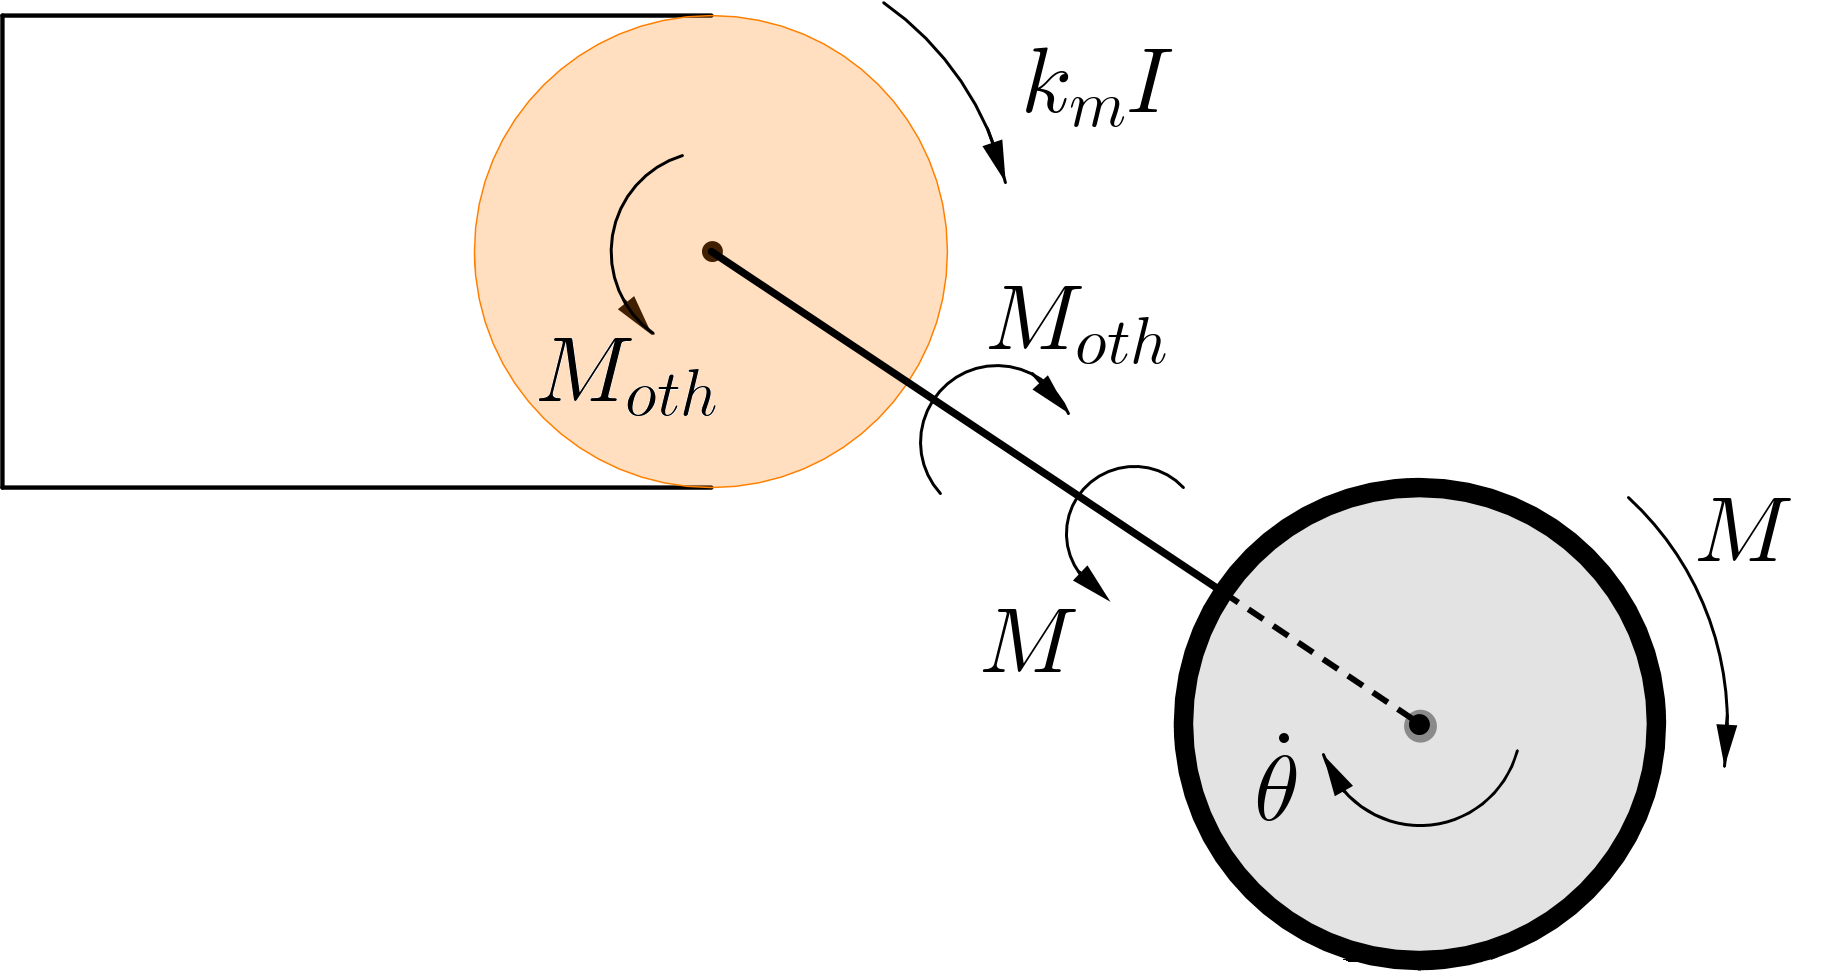
\includegraphics[scale=1]{for_M.png} }
	\caption{Передача силового воздействия с мотора на колеса.}
	\label{for_M}
\end{figure}

Согласно рис.~\ref{for_M}, на колеса с моментом $M$ действует стержень, соединяющий их с валом мотора.
В~свою очередь колеса действуют на него с таким же моментом, направленным в противоположную сторону\lefteqn.\footnote{В~данном случае это напрямую следует из третьего закона Ньютона.}
Стержень и вал сервопривода действуют друг на друга с моментом $M_{oth}$.
В~результате, записав для вращательного движения указанных тел соответствующие уравнения, получим\footnote{Перед $M_{oth}$ в приводимых уравнениях в отличие от~\eqref{servo} поставлен минус по той причине, что теперь под ним мы понимаем конкретный момент сил, а не используем $M_{oth}$ как некоторое обобщающее обозначение.}:
\begin{align}
	&k_mI - M_{oth} = J\ddot\theta, &&\text{(для вала мотора)}\\
	&M_{oth} - M = J_{o}\ddot\theta, &&\text{(для соединительного стержня)}	
\end{align}
где $J_{o}$~--- момент инерции соединительного стержня.
Из полученных уравнений, полагая $J_o = 0$ по причине его малости, несложно получить, что 
\begin{equation}
	M_{oth} = M,
\end{equation}
а значит
\begin{equation}
	M = k_mI-J\ddot\theta\ldotp
\end{equation}

Выражение для силы тока следует взять из второй работы:
\begin{equation}
	IR = U - k_e\dot\theta - L_\textit{р}\dot{I},
\end{equation}
где $U = U_{ctrl}$.
Из него, пренебрегая в силу ее малости индуктивностью, получим
\begin{equation}
	I = \frac{U-k_e\dot\theta}{R}\ldotp
\end{equation}
Выражение для $M$ в таком случае запишется в виде
\begin{equation}\label{ftr}
	M = \frac{k_m}{R}\left(U-k_e\dot\theta\right) - J\ddot\theta\ldotp
\end{equation}

Подставим полученное выражение в нашу систему~\eqref{final_in_mech}:
\begin{equation}
	\left\{  
	\begin{aligned}
		\!&\left(m_pl^2 + 4J_p\right)\ddot\psi + 2m_plr\ddot\theta\cos\psi - 2m_pgl\sin\psi= 0\\
		\!&\begin{split}0.5m_plr\ddot\psi\cos\psi + &\left(m_pr^2 + m_cr^2 + 4m_wr^2 + 4J_w\right)\ddot\theta -\\ 	
			&\phantom{--------}-0.5m_plr\dot\psi^2\sin\psi = \frac{2k_m}{R}\left(U-k_e\dot\theta\right) - 2J\ddot\theta\ldotp
		\end{split}	
	\end{aligned}   
	\right.
\end{equation}
и перепишем ее в виде
\begin{equation}\label{final_in_all}
	\left\{  
	\begin{aligned}
		\!&\left(m_pl^2 + 4J_p\right)\ddot\psi + 2m_plr\ddot\theta\cos\psi - 2m_pgl\sin\psi= 0\\
		\!&\begin{split}0.5m_plr\ddot\psi\cos\psi + &\left(m_pr^2 + m_cr^2 + 4m_wr^2 + 4J_w + 2J\right)\ddot\theta - \\	
			&\phantom{----------}-0.5m_plr\dot\psi^2\sin\psi + \frac{2k_mk_e}{R}\dot\theta = \frac{2k_m}{R}U\ldotp
		\end{split}	
	\end{aligned}   
	\right.
\end{equation}

В~лице данной системы мы получили математическую модель рассматриваемого робота, то есть совокупность уравнений, описывающих все протекающие в нем механические и электродинамические процессы.
Из сказанного следует, что в общем виде задача данного раздела решена.
Несмотря на это, прежде, чем его завершить, следует сделать еще пару немаловажных вещей.

Во-первых, можно видеть, что в уравнениях~\eqref{final_in_all} присутствуют сложные зависимости от величин $\psi$ и $\theta$, а также от их производных.
Это неоправданно сильно затрудняет техническую реализацию робота, поэтому модель следует упростить.
Легчайший способ сделать это видится в том, чтобы линеаризовать полученные уравнения, то есть сделать все зависимости от указанных функций линейными, что мы и сделаем.

Учитывая, что при малых углах (выраженных в радианах) приближенно выполняются следующие равенства:
\begin{align}
	\sin\alpha &= \alpha, & \cos\alpha = 1,
\end{align}
сделаем соответствующие замены в~\eqref{final_in_all}:
\begin{equation}\label{final_in_all_but_easier}
	\left\{  
	\begin{aligned}
		\!&\left(m_pl^2 + 4J_p\right)\ddot\psi + 2m_plr\ddot\theta - 2m_pgl\psi = 0\\
		\!&0.5m_plr\ddot\psi + \left(m_pr^2 + m_cr^2 + 4m_wr^2 + 4J_w + 2J\right)\ddot\theta - 	
			0.5m_plr\dot\psi^2\psi + \frac{2k_mk_e}{R}\dot\theta = \frac{2k_m}{R}U\ldotp
	\end{aligned}   
	\right.
\end{equation}
Учитывая, что при перемножении двух и более чисел, по модулю меньших единицы, абсолютное значение итогового результата еще более уменьшается, положим в~\eqref{final_in_all_but_easier} все квадраты и взаимные произведения величин $\psi$ и $\theta$ (и их производных) равными нулю:
\begin{equation}\label{final_in_all_but_the_easiest}
	\left\{  
	\begin{aligned}
		\!&\left(m_pl^2 + 4J_p\right)\ddot\psi + 2m_plr\ddot\theta - 2m_pgl\psi = 0\\
		\!&0.5m_plr\ddot\psi + \left(m_pr^2 + m_cr^2 + 4m_wr^2 + 4J_w + 2J\right)\ddot\theta	
			 + \frac{2k_mk_e}{R}\dot\theta = \frac{2k_m}{R}U\ldotp
	\end{aligned}   
	\right.
\end{equation}

Таким образом, мы упростили нашу математическую модель и сделали ее более доступной для технической реализации.
Теперь упростим ее для дальнейших математических расчетов, переписав в определенном матричном виде.

Введем следующие обозначения:
\begin{gather}
	q = 
	\begin{bmatrix}
		\theta\\
		\psi
	\end{bmatrix}\!\!, 
	\\
	u = U.
\end{gather}
С~учетом их можно записать систему~\eqref{final_in_all_but_the_easiest} в виде
\begin{equation}
	E\ddot{q} + F\dot{q} + Gq = Hu
\end{equation}
где
\begin{gather}
	E = 
	\begin{bmatrix}
		2m_plr & m_pl^2 + 4J_p\\
		m_pr^2 + m_cr^2 + 4m_wr^2 + 4J_w + 2J & 0.5m_plr
	\end{bmatrix}\!\!,\;
	F = 
	\begin{bmatrix}
		0 & \phantom{!}0\phantom{!}\\
		\cfrac{2k_mk_e}{R} & 0
	\end{bmatrix}\!\!,\;
	G =
	\begin{bmatrix}
		0 & -2m_pgl\\
		\phantom{!}0\phantom{!} & 0	
	\end{bmatrix}\!\!,\notag\\
	H = 
	\begin{bmatrix}
		0\\
		\cfrac{2k_m}{R}
	\end{bmatrix}\!\!,\qquad
	\dot{q} =
	\begin{bmatrix}
		\dot{\theta}\\
		\dot{\psi}
	\end{bmatrix}\!\!,\qquad
	\ddot{q} =
	\begin{bmatrix}
		\ddot{\theta}\\
		\ddot{\psi}
	\end{bmatrix}\!\!\ldotp			 
\end{gather}
Теперь выразим из полученного уравнения матрицу $\ddot{q}$, умножив все выражение на матрицу $E^{-1}$ слева и перебросив некоторые слагаемые  в другую часть уравнения:
\begin{equation}
	\ddot{q}=-E^{-1}F\dot{q} - E^{-1}Gq + E^{-1}Hu,
\end{equation}
где
\begin{gather}
	E^{-1} = 
	\begin{bmatrix}
		\cfrac{0.5m_plr}{\varkappa_1} & -\cfrac{m_pl^2 + 4J_p}{\varkappa_1}\\
		-\cfrac{r^2(m_p + m_c + 4m_w) + 4J_w + 2J}{\varkappa_1} & \cfrac{2m_plr}{\varkappa_1}
	\end{bmatrix}\!\!,\;
	E^{-1}F = 
	\begin{bmatrix}
		-\cfrac{2k_mk_e\left(m_pl^2 + 4J_p\right)}{R\varkappa_1} & \phantom{!}0\phantom{!}\\
		\cfrac{4k_mk_em_plr}{R\varkappa_1} & 0
	\end{bmatrix}\!\!,\;\notag\\
	E^{-1}G = 
	\begin{bmatrix}
		\phantom{!}0\phantom{!} & -\cfrac{m_p^2gl^2r}{\varkappa_1}\\
		0 & \cfrac{2m_pgl\left(r^2(m_p + m_c + 4m_w) + 4J_w + 2J\right)}{\varkappa_1}
	\end{bmatrix}\!\!,\;
	E^{-1}H = 
	\begin{bmatrix}
		-\cfrac{2k_m\left(m_pl^2 + 4J_p\right)}{R\varkappa_1} \\
		\cfrac{4k_mm_plr}{R\varkappa_1} 
	\end{bmatrix}\!\!,
\end{gather} 
где, в свою очередь,
\begin{equation}
	\varkappa_1 = m_p^2l^2r^2 - \left(m_pl^2 + 4J_p\right)\left(r^2(m_p + m_c +
	 4m_w)+4J_w + 2J\right)\ldotp
\end{equation}
Приводя получившееся выражение обратно в форму системы, получим
\begin{equation}
	\left\{  
	\begin{aligned}
		\!&\ddot\theta = \cfrac{2k_mk_e\left(m_pl^2 + 4J_p\right)}{R\varkappa_1}\,\dot\theta +
		\cfrac{m_p^2gl^2r}{\varkappa_1}\,\psi 
		-\cfrac{2k_m\left(m_pl^2 + 4J_p\right)}{R\varkappa_1}\,U\\
		%
		\!&\ddot\psi = -\cfrac{4k_mk_em_plr}{R\varkappa_1}\,\dot\theta -
		\cfrac{2m_pgl\left(r^2(m_p + m_c + 4m_w) + 4J_w + 2J\right)}{\varkappa_1}\,\psi +
		\cfrac{4k_mm_plr}{R\varkappa_1}\,U.
	\end{aligned}   
	\right.
\end{equation}
Для того чтобы теперь окончательно перейти к тому виду математической модели, который нам нужен, добавим в нее еще одно глупое, но заведомо верное уравнение:
\begin{equation}\label{math_model}
	\left\{  
	\begin{aligned}
		\!& \dot{\psi} = \dot{\psi} \\
		\!&\ddot\theta = \cfrac{2k_mk_e\left(m_pl^2 + 4J_p\right)}{R\varkappa_1}\,\dot\theta +
		\cfrac{m_p^2gl^2r}{\varkappa_1}\,\psi 
		-\cfrac{2k_m\left(m_pl^2 + 4J_p\right)}{R\varkappa_1}\,U\\
		%
		\!&\ddot\psi = -\cfrac{4k_mk_em_plr}{R\varkappa_1}\,\dot\theta -
		\cfrac{2m_pgl\left(r^2(m_p + m_c + 4m_w) + 4J_w + 2J\right)}{\varkappa_1}\,\psi +
		\cfrac{4k_mm_plr}{R\varkappa_1}\,U.
	\end{aligned}   
	\right.
\end{equation}
В~этом случае введя обозначение
\begin{equation}
	x =
	\begin{bmatrix}
		\psi \\
		\dot{\theta} \\
		\dot{\psi}
	\end{bmatrix}\!\!,
\end{equation}
математическую модель нашего робота можно записать в виде
\begin{equation}
	\dot x = Ax + Bu,
\end{equation}
где 
\begin{gather}
	A =
	\begin{bmatrix}
		0 & 0 & \phantom{!}1\phantom{!} \\
		\cfrac{m_p^2gl^2r}{\varkappa_1} & \cfrac{2k_mk_e\left(m_pl^2 + 4J_p\right)}{R\varkappa_1}& 0\\
		-\cfrac{2m_pgl\left(r^2(m_p + m_c + 4m_w) + 4J_w + 2J\right)}{\varkappa_1} &
		 -\cfrac{4k_mk_em_plr}{R\varkappa_1} & 0
	\end{bmatrix}\!\!\\
	B = 
	\begin{bmatrix}
		0 \\
		-\cfrac{2k_m\left(m_pl^2 + 4J_p\right)}{R\varkappa_1} \\
		\cfrac{4k_mm_plr}{R\varkappa_1}
	\end{bmatrix}\!\!\ldotp
\end{gather}
\paragraph*{Схема моделирования работы механизма}$\phantom{-}$\\
\hspace*{\parindent}Схема моделирования исследуемого робота, построенная на основании его математической модели (уравнения~\eqref{math_model}) будет иметь вид, показанный на рис.~\ref{struct_sheme}.

\begin{figure}[h]
	\noindent\centering{ 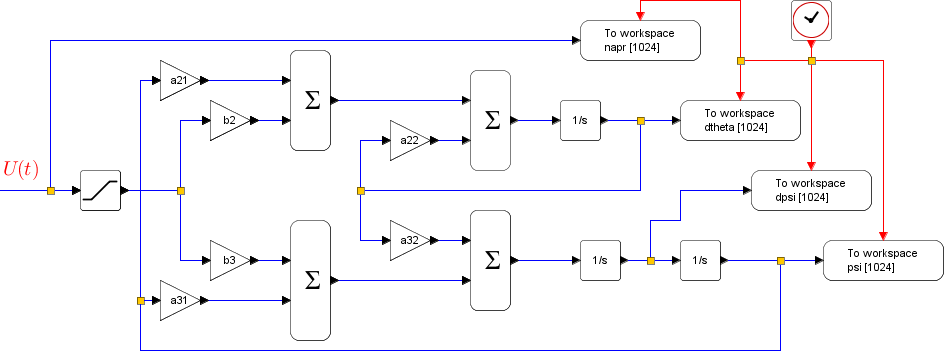
\includegraphics[scale=0.7]{struct_sheme.png} }
	\caption{Схема моделирования работы устройства.}
	\label{struct_sheme}
\end{figure}

Расшифровка входящих в нее переменных такова:
\begin{align}
	a22 &= \frac{2k_mk_e\left(m_pl^2 + 4J_p\right)}{R\varkappa_1} & 
	a32 &= -\frac{4k_mk_em_plr}{R\varkappa_1}\notag \\
	a21 &= \frac{m_p^2gl^2r}{\varkappa_1} & 
	a31 &= -\cfrac{2m_pgl\left(r^2(m_p + m_c + 4m_w) + 4J_w + 2J\right)}{\varkappa_1} \\
	b2 &= -\frac{2k_m\left(m_pl^2 + 4J_p\right)}{R\varkappa_1} & 
	b3 &= \cfrac{4k_mm_plr}{R\varkappa_1} \notag
\end{align}

Используя схему моделирования нашего устройства, мы имеем своей целью при известной зависимости $U(t)$ и при заданных начальных условиях~--- значениях функций $\psi(t)$, $\dot{\psi}(t)$ и $\dot{\theta}(t)$ в момент времени $t=0$~--- определить дальнейшее поведение робота.
Под нахождением последнего подразумевается, что в результате моделирования нам станут известны значения тех характеризующих состояние механизма величин, которые входят в его математическую модель.
В~данном случае их роль играют $\psi$, $\dot{\theta}$ и $\dot{\psi}$.

Четыре регистрирующих блока с надписью To~Workspace нужны (соответственно сверху вниз) для фиксации значений $U$, $\dot{\theta}$, $\dot{\psi}$ и $\psi$.
Входящие в эту схему блоки, помеченные значком $\sum$, на выходе выдают сумму своих входных сигналов.

Разобраться в строении схемы моделирования помогут уравнения математической модели, записанные немного в другом виде~--- см.~систему~\eqref{integral}.
 
\begin{equation}\label{integral}
	\left\{  
	\begin{aligned}
		\!&\psi = \int\dot{\psi}\,dt\\
		\!&\dot\theta = \int\left(\cfrac{2k_mk_e\left(m_pl^2 + 4J_p\right)}{R\varkappa_1}\,\dot\theta +
		\cfrac{m_p^2gl^2r}{\varkappa_1}\,\psi 
		-\cfrac{2k_m\left(m_pl^2 + 4J_p\right)}{R\varkappa_1}\,U\right)\,dt\\
		%
		\!&\dot\psi = \int\left(-\cfrac{4k_mk_em_plr}{R\varkappa_1}\,\dot\theta -
		\cfrac{2m_pgl\left(r^2(m_p + m_c + 4m_w) + 4J_w + 2J\right)}{\varkappa_1}\,\psi +
		\cfrac{4k_mm_plr}{R\varkappa_1}\,U\right)\,dt.
	\end{aligned}   
	\right.
\end{equation}

Эту же схему моделирования можно представить и более компактно. Результат -- см. рис.~\ref{struct_sheme_with_2_sums}. По сравнению с прошлой в этой ее версии опущены два лишних сумматора.

\begin{figure}[h]
	\noindent\centering{ 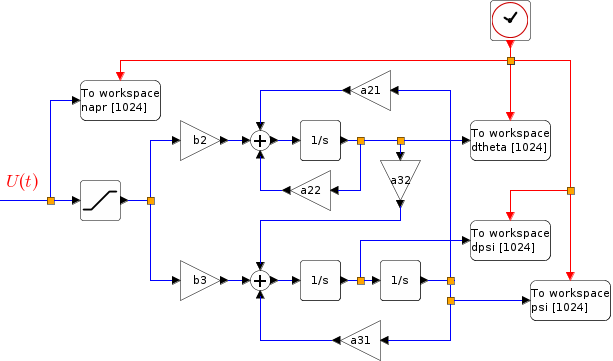
\includegraphics[scale=1]{struct_sheme_with_2_sums.png} }
	\caption{Схема моделирования работы устройства в более компактной форме.}
	\label{struct_sheme_with_2_sums}
\end{figure}
 
\end{document}
